\chapter{Models and Discretization}

In this chapter, the mathematical description of the multi-scale model and its discretization is presented. 
We use the multi-scale chemo-electro-mechanical model that was introduced in literature \cite{Roehrle2012,Heidlauf2013,Heidlauf2015Diss,Mordhorst2015}. Additional models known from literature are incorporated that  were previously only simulated in isolation: The multidomain description for electrophysiology \cite{Klotz2020}, a model of neural stimulation \cite{Cisi2008} and sensory organ models such as the muscle spindle model of Mileusnic et al. \cite{Mileusnic2006Spindle}. Similarly, models of Golgi tendon organs can be added \cite{Mileusnic2006Golgi}.

% components of the multi-scale model
\begin{figure}%
  \centering%
  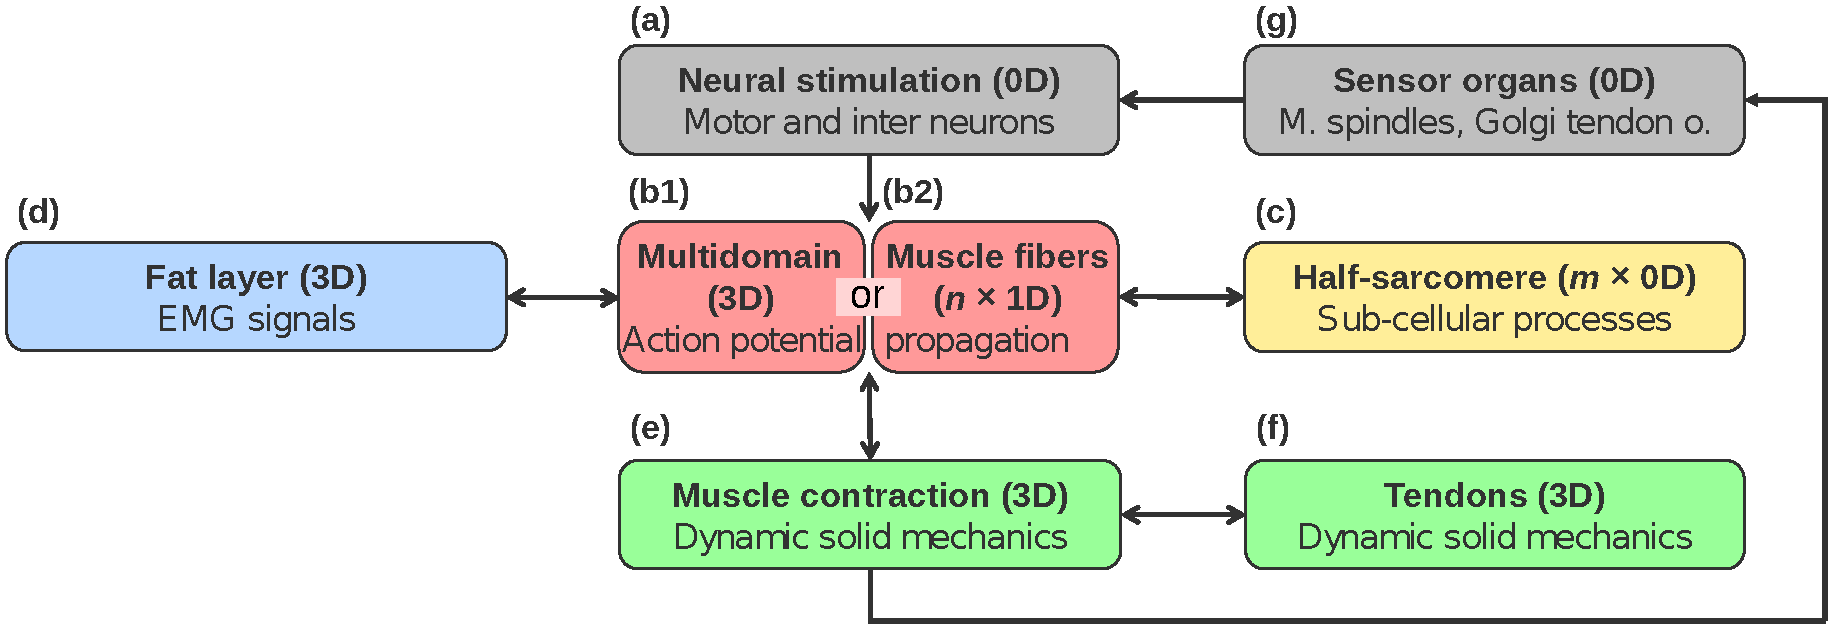
\includegraphics[width=\textwidth]{images/theory/model_schematic.pdf}%
  \caption{Interacting components of the multi-scale model.}%
  \label{fig:multi-scale-model}%
\end{figure}

\Cref{fig:multi-scale-model} shows an overview of the components of the implemented multi-scale model.
A pool of motor neurons drives the stimulation of the muscular system in \cref{fig:multi-scale-model} (a). 
The axons of each motor neuron innervate the muscle fibers corresponding to the same MU and transmit rate-encoded stimulation signals.

In the muscle tissue, action potentials propagate starting at the neuromuscular junctions and subsequently reach the whole length of the muscle.
In our multi-scale model, two different formulations are available to describe this phenomenon. The multidomain description (\cref{fig:multi-scale-model} (b1)) models the MUs from a  homogenized 3D perspective. The description with muscle fibers (\cref{fig:multi-scale-model} (b2)) models action potential propagation explicitely with $n$ 1D muscle fibers. 

Both of these descriptions of electrophysiology involve a subcellular model (\cref{fig:multi-scale-model} (c)). This model describes the ionic processes involving the fiber membranes and taking place within one half of a sarcomere as the smallest unit to generate muscle forces. A large number $m$ of instances of this model has to be computed. 

In addition to the physiology of the muscle, a layer of body fat and skin on top of the muscle belly can be added to the model. This 3D fat layer (\cref{fig:multi-scale-model} (d)) is used to simulate EMG recordings on the skin surface. The model for the fat layer is unidirectionally coupled with the muscle fiber model (\cref{fig:multi-scale-model} (b2)) or bidirectionally coupled with the multidomain model (\cref{fig:multi-scale-model} (b1)). Using the multidomain model, it is, thus, possible to simulate external stimulation by electrodes on the skin, which is subject to research in neuroprosthetics.

The activated muscle generates force by subcellular proceses on a molecular scale. They are computed on the cellular level by the half-sarcomere model (c). On the macroscopic scale, stresses lead to strains and contraction of the muscle. This effect is described by the muscle contraction model on a 3D domain (\cref{fig:multi-scale-model} (e)). 
The description is coupled with the electrophysiology models (b1),(b2) by the geometry of the contracting muscle and fibers. It is coupled with the subcellular model by the generated active stresses of the half-sarcomere. Displacements and stresses can be computed for the muscle belly itself, but also for the connected body fat layer and for elastic tendons (\cref{fig:multi-scale-model} (f)). Depending on the research questions, the contraction model is either formulated quasi-static or fully dynamic taking into account inertia effects.

Sensory organs such as muscle spindles and Golgi tendon organs sense fiber stretch and contraction velocity (\cref{fig:multi-scale-model} (g)). They are connected with the motor neuron pool by layers of interneurons and modulate the stimulation in \cref{fig:multi-scale-model} (a).

In this chapter, \cref{sec:model_equations} presents mathematical descriptions of all model components in the multi-scale framework and \cref{sec:discretization} addresses their discretization in time and space. An own section, \cref{sec:discretization_mechanics}, is dedicated to the discretization and solution of the mechanics model.

\section{Model Equations}\label{sec:model_equations}
In the following, more details and mathematical descriptions are given for the outlined models. The section begins with the 0D half-sarcomere model in \cref{sec:subcelullar_model}, followed by the bidomain and monodomain models in \cref{sec:bidomain_model,sec:monodomain_model}, which constitute the muscle fiber based model of electrophysiology. \Cref{sec:multidomain_model} continues with the multidomain model. Electric conduction in the body fat layer is described in \cref{sec:electric_conduction_body_domain}. An overview of the continuum mechanics model used for muscle contraction is given in \cref{sec:model_muscle_contraction}.
% ----------
\subsection{Subcellular Model}\label{sec:subcelullar_model}

Propagation of electric stimuli along muscle fibers involves activation and deactivation of ion channels and ion pumps in the fiber membrane  (the sarcolemma) and in the transverse tubules.
Functioning of these processes on the subcellular scale have first been suggested in 1952 by Hodgkin and Huxley after their studies of the squid giant axons \cite{Hodgkin1952,hodgkin1952propagation}. To date, their mathematical model still serves as the basis for electrophysiology models and some of their predictions, e.g., on gating currents that occur during opening of channels, were experimentally confirmed later.

The fiber membrane separates intra- and extracellular space and can be locally described by an electric circuit. The membrane voltage $V_m=\phi_i-\phi_e$ is the difference between the intra and extracellular potentials $\phi_i$ and $\phi_e$. The membrane stores charges $Q$, quantifiable by its electric capacitance $C_m$:
\begin{align}\label{eq:subcellular_model_helper1}
  Q = C_m\cdot V_m.  
\end{align}
%
A change in the transmembrane potential, e.g., induced by an action potential leads to a change in $Q$, which is accounted for by an electric current $I$ over the membrane. This can be formally obtained by the derivative of \cref{eq:subcellular_model_helper1} with respect to time:%
\begin{align}\label{eq:subcellular_model_helper2}
  \d{Q}{t} = C_m \cdot \d{V_m}{t}.
\end{align}
%
The current $I=\d Q / \d t$ is realized by ions passing through the membrane.
Significant ions in this process are sodium $(\text{Na}^{+})$ and potassium ions $(\text{K}^{+})$.
Considering a particular point on the fiber, these ions diffuse through ion-specific channels in the membrane.
The diffusion is driven by an interplay of the ion concentration gradient and the electric field that is caused by action potentials.

Without any electric field imposed by action potentials, the equilibrium state of the diffusion process for sodium and potassium ions is given by their Nernst potentials $E_{\text{Na}^{+}}$ and $E_{\text{K}^{+}}$. These voltage levels depend on logarithmic relations between extra- and intracellular concentrations scaled by constants describing the thermic energy and the number of electrons.
In thermodynamic equilibrium, the membrane voltage is equal to the Nernst potential $E_i$ of the involved ions $i$. 
At a higher membrane voltage $V_m$, the remainder ($V_m - E_i$) is the part of the electric field that drives the
ion fluxes and electric currents through the membrane. The currents depend on the conductivity $g_i$ of
the membrane for ion $i$. 

Apart from sodium and potassium ions, the diffusion of less frequent ions and ionic pumps can be lumped by a leakage current $I_L$ that is modeled by a channel with constant conductivity $\bar{g}_L$.
With this, the total ionic membrane current $I_\text{ion}$ is formulated as
%
\begin{subequations}
\begin{align}\label{eq:subcellular_model_helper4}
  I_\text{ion}(V_m)  &= I_{\text{Na}^{+}} + I_{\text{K}^{+}} + I_L \\
  & = g_{\text{Na}^{+}}\,(V_m - E_{\text{Na}^{+}}) + g_{\text{K}^{+}}\,(V_m - E_{\text{K}^{+}}) + \bar{g}_L\,(V_m - E_L). \label{eq:subcellular_model_helper5}
\end{align}
\end{subequations}
%
The conductivities $g_{\text{Na}^{+}}$ and $g_{\text{K}^{+}}$ for the sodium and potassium channels depend on the transmembrane voltage $V_m$ and its history.

In addition to the ionic current $I_\text{ion}$, an externally driven current $I_\text{ext}$ can be modeled that occurs as a result of neural stimulation at the neuromuscular junctions. Substituting the current $I=\d Q / \d t$ in \cref{eq:subcellular_model_helper2}, we get the following differential equation for the membrane voltage $V_m$:
\begin{align}\label{eq:subcellular_model_helper3}
  C_m \cdot \d{V_m}{t} = -I_\text{ion}(V_m) + \dfrac{I_\text{ext}}{A}.
\end{align}
%
The negative sign of the ionic current $I_\text{ion}$ is in accordance with the definition of the membrane voltage as $V_m=\phi_i-\phi_e$. The external current $I_\text{ext}$ is divided by the surface area $A$ of the stimulating electrode or neuromuscular junction, as the description considers an infinitesimal area on the membrane.

Hodgkin and Huxley suggested that ion channels can be activated and deactivated. This molecular process requires independent \say{gating} particles to move to a new position in order for a channel to be activated. For the potassium channel, four of these independent events have to occur, each modeled by a propability $n$. The resulting probability for the channel to open is, thus, $n^4$. For the sodium channel, three such events are assumed for activation and another one for the deactivation of the channel, described by the propabilities $m$ and $h$, respectively. The values of the probabilities change over time and modulate the conductivities of the ion channels:
%
\begin{align*}
  g_{\text{Na}^{+}} &= \bar{g}_{\text{Na}^{+}} \cdot m(t)^3 \cdot h(t), \quad &g_{\text{K}^{+}} &= \bar{g}_{\text{K}^{+}} \cdot n(t)^4.
\end{align*}
%
Here, $\bar{g}_{\text{Na}^{+}}$ and $\bar{g}_{\text{K}^{+}}$ are channel specific constants. The gating variables $n,m$ and $h$ can be interpreted as probabilities for the events to occur or as the amount of occured events related to all available gating particles. 
The evolution of the activation probability $n$ is modeled by the following ordinary differential equation (ODE):%
\begin{align*}
  \d{n}{t} = \alpha_n(V_m) \cdot (1-n) + \beta_n(V_m) \cdot n,
\end{align*}
analogously for $h$ and $n$. The transition rates between activation probability $n$ and deactivation probability $(1-n)$ are nonlinearly dependent on the membrane voltage $V_m$.

For a constant $V_m$, this ODE has an analytical solution
\begin{align}\label{eq:subcellular_model_helper0}
  n(t) = n_\infty\big(1 - \exp(1 - \dfrac{1}{\tau_n}t)\big),
\end{align}
which for $t\to \infty$ converges to the equilibrium value $n_\infty := \alpha_n\,\tau_n$ as shown in \cref{fig:ode_solution}. The time constant $\tau_n := 1/(\alpha_n + \beta_n)$ indicates how fast the solution approaches the equilibrium, e.g., when starting from $n(0)=0$, half of the value of the equilibrium is reached after $t_{1/2}=\log(2)\,\tau_n$. The smaller $\tau_n$, the stiffer is the ODE, which needs to be considered in the choice of a suitable numerical solution scheme.

\begin{figure}%
  \centering%
  \def\svgwidth{0.4\textwidth}
  \input{images/theory/ode_solution.pdf_tex}%
  \caption{Subcellular model: Graph of the analytic solution (red) of the ordinary differential equation that is part of the activation model of ion channels for constant transmembrane voltage and initial condition $n(0)=0$, given in \cref{eq:subcellular_model_helper0}. The variables $n_\infty$ and $\tau_n$ can be interpreted as the equilibrium value and a characteristic time scale, respectively.}%
  \label{fig:ode_solution}%
\end{figure}

Because the transmembrane voltage $V_m$ changes over time, the ODEs for $n, m$ and $h$ have to be solved numerically. Then, the dependent ionic current $I_\text{ion}$ can be calculated. Thus, the model is a system of differential-algebraic equations (DAE).

The internal states in this model can be combined into a state vector $\bfy = (n,m,h)^\top$. 
The combined right hand side for all states is formulated as a vector-valued function $G(V_m,\bfy)$.
In summary, the system of DAEs for the subcellular model on a subcellular domain $\Omega_s$ can be written in the following form:
\begin{align}
  \dfrac{\partial\bfy}{\partial t} &= G(V_m,\bfy),& I_\text{ion}&=I_\text{ion}(V_m,\bfy) \quad \text{on }\Omega_s\label{eq:subcellular}.
\end{align}
For an exemplary solution that shows how the membrane potential changes over time, see \cref{fig:action_potentials}. 

The system of equations in \cref{eq:subcellular} together with \cref{eq:subcellular_model_helper3} describe the subcellular processes on a single point $\Omega_s \subset \Omega_f$ on a muscle fiber $\Omega_f$. 
It does not model the interaction between neighboring points that leads to propagation of action potentials.
To account for action potential propagation, ionic currents $I_\text{ion}$ on multiple points are coupled within the multidomain or fiber models that are formulated in the multi-scale framework. This is described in the following sections, \cref{sec:bidomain_model,sec:monodomain_model,sec:multidomain_model}.
Using these models, the system of ODEs in \cref{eq:subcellular} has to be solved for multiple subcellular points $\Omega_s^i$ in the muscle domain.

After Hodgkin and Huxley proposed this model in 1952, more detailed models were formulated that take into account more ion channels, ion pumps and more advanced biochemical processes within the cell. One particular model is the one proposed by Shorten et al. \cite{Shorten2007}, which adds the full pathway from activation to excitation-contraction coupling in the sarcomere. It has a state vector of $\bfy \in \R^{56}$ and is used to compute active stresses for simulations of muscle contraction. 
It can also be written in the form given in \cref{eq:subcellular}.
Apart from $I_\text{ion}$, another value $\gamma = H(\bfy,\dot{\lambda}_f)$ is computed by an additional equation from the vector of states $\bfy$ and the fiber contraction velocity $\dot{\lambda}_f$, which is given to the model as a parameter.
The value $\gamma$ is a lumped activation parameter in the range $\gamma \in [0,1]$ that describes the amount of active stress generated in the sarcomere and can be linked to the continuum mechanics model of muscle contraction.

%and alter the ion concentration gradients across the membrane.
%ion-specific channels
%electrochemical gradient
%channels respond to a change in transmembrane potential 
%altered ion concentration gradients

% ----------
\subsection{Bidomain Model}\label{sec:bidomain_model}

A description of electrophysiology on a general 3D muscle tissue is given by the bidomain model formulated by \cite{tung1978bi,peskoff1979electric}. The bidomain model considers the intra (index $i$) and extracellular spaces (index $e$) in a homogenized setting, such that the two domains coexist at every spatial point $\bfx \in \Omega\subset \R^3$. Similar to the setting of the subcellular model, the two domains in the bidomain model have locally varying electric potential fields $\phi_i$ and $\phi_e$ that yield a locally varying transmembrane voltage $V_m=\phi_i - \phi_e$. Electric conduction within the two domains is governed by conductivity tensors $\bfsigma_i$ and $\bfsigma_e$. 

Assuming static conditions, a spatially varying electric potential $\phi$ induces the electric field $E=-\grad \phi$.
According to Ohm's law, the resulting current density $j$ is given by 
%
\begin{align}\label{eq:bidomain_helper1}
  j = \bfsigma\,E = -\bfsigma\,\grad \phi \quad \text{in }\Omega.
\end{align}
This holds for both intra and extracellular domain, yielding expressions for $j_i$ and $j_e$.

The intracellular and the extracellular domain are electrochemically coupled. Thus, one assumption is that currents are preserved and a change in current density on one domain corresponds to the opposite change in current density in the other domain. This is expressed by the divergence of the current densities, which in one domain equals to the negated value in the other domain:
%
\begin{align}\label{eq:bidomain_helper2}
  \div(j_i) = -\div(j_e) \quad \text{in }\Omega.
\end{align}
%
This change in current density directly corresponds to a current flow over the membrane:%
%
\begin{align*}
  \div(j_i) = A_m\,I_m \quad \text{in }\Omega.
\end{align*}
%
Here, the factor $A_m$ describes the membrane area to domain volume relationship. It is needed to convert the units between current per volume and current per area. The membrane current $I_m$ is given by the subcellular model of Hodgkin and Huxley in \cref{eq:subcellular_model_helper3}. Neglecting the external current $I_\text{ext}$ in \cref{eq:subcellular_model_helper3} and using the formulation of the intracellular current density $j_i$ in \cref{eq:bidomain_helper1}, we get:
%
\begin{align*}
  \div\big(\bfsigma_i\,\grad(\phi_i)\big) = A_m\,\big(C_m\,\p{V_m}{t} + I_\text{ion}(V_m)\big) \quad \text{in }\Omega.
\end{align*}
%
The ionic current $I_\text{ion}$ can be computed by \cref{eq:subcellular_model_helper5}. 
By plugging \cref{eq:bidomain_helper1} also into \cref{eq:bidomain_helper2} and rewriting the equations in terms of the extracellular potential $\phi_e$ and the transmembrane voltage $V_m = \phi_i-\phi_e$, we get the bidomain equations:%
\begin{subequations}
  \begin{align}
    \div\big((\bfsigma_i + \bfsigma_e)\,\grad(\phi_e)\big) + \div(\bfsigma_i\,\grad(V_m)\big) &= 0,\label{eq:bidomain1} \\[4mm]
    \div\big(\bfsigma_i\,\grad(V_m)\big) + \div(\bfsigma_i\,\grad(\phi_e)\big) &= A_m\,\big(C_m\,\p{V_m}{t} + I_\text{ion}(V_m)\big).  \label{eq:bidomain2}
  \end{align}
\end{subequations}
%
With appropriate boundary conditions, these equations are often used to model cardiac electrophysiology. They also serve as a basis for the fiber models in our multi-scale setting, which will be described in the next section.

% ----------
\subsection{Monodomain Model}\label{sec:monodomain_model}
% ----------
One approach to modeling skeletal muscle electrophysiology is to explicitly resolve muscle fibers and compute propagating action potentials on these spatial domains.
Propagation of action potentials can be described by the monodomain equation, which is a specialization of the bidomain equations for a one-dimensional intracellular space.

We assume a muscle domain $\Omega_M \subset \R^3$ with a number of embedded 1D manifolds $\Omega_f^j\subset \R^3$ for $j=1,\dots,n$ that represent muscle fibers. The domain $\Omega_M$ represents the extracellular space and each fiber domain $\Omega_f^j$ represents a separate  intracellular space.
It is further assumed that electric conduction in the extracellular space is directed equally to the embedded fibers. This can be stated as%
\begin{align}\label{eq:monodomain_helper1}
  \bfsigma_i = k\cdot \bfsigma_e.  
\end{align}
%
The intracellular conductivity tensor $\bfsigma_i$ (here prolonged from the scalar value $\sigma_i$ on a fiber with tangent $\bfa \in \R^3$ to the 3D domain by $\bfsigma_i = \sigma_i \, \bfa \otimes \bfa$) and the extracellular conductivity $\bfsigma_e$ are multiples of each other with a scaling factor $k\in\R$.

Plugging \cref{eq:monodomain_helper1} into the first bidomain equation, \cref{eq:bidomain1}, and restricting the domain to a 1D fiber $\Omega_f^j$ allows to combine the terms related to $\phi_e$:
%
\begin{align*}
  \div\big(\sigma_i\,\grad(\phi_e)\big) = -\dfrac{k}{k+1} \div\big(\sigma_i\,\grad(V_m)\big) \quad \text{on }\Omega_f^j.
\end{align*}
% 
Using the second bidomain equation, \cref{eq:bidomain2}, we get the expression
%
\begin{align*}
  \div\big(\sigma_\text{eff} \,\grad(V_m)\big) = A_m\big(C_m\,\p{V_m}{t} + I_\text{ion}(V_m,\bfy)\big) \quad \text{on }\Omega_f^j.
\end{align*}
%
The effective conductivity $\sigma_\text{eff}$ combines the intra and extracellular conductivities, $\sigma_i$ and $\sigma_e$, analogous to a parallel circuit:
\begin{align*}
  \sigma_\text{eff} := \sigma_i \parallel \sigma_e = \dfrac{\sigma_i\,\sigma_e}{\sigma_i + \sigma_e}.
\end{align*}
%
Rearranging the terms yields the classical form of the monodomain equation:
%
\begin{align}
  &\dfrac{\partial V_m}{\partial t} = \dfrac{1}{A_m\,C_m}\big(\sigma_\text{eff}\dfrac{\partial^2 V_m}{\partial x^2} - A_m\,I_\text{ion}(V_m,\bfy)\big) \quad && \text{for }x \in \Omega_f^j. \label{eq:monodomain}
\end{align}
%

The multi-scale framework uses multiple instances of the monodomain equation \\\cref{eq:monodomain} together with the first bidomain equation \cref{eq:bidomain1} to model electrophysiology in the fibers and the extracellular domain \cite{Mordhorst2015}. In addition to the fiber domains $\Omega_f^j$, two instances of the muscle domain $\Omega_M$ are needed for the bidomain equation, one for the intracellular and one for the extracellular space. The transmembrane potential $V_m$ is unidirectionally coupled from the fiber meshes to the intracellular space of the first bidomain equation. The extracellular potential $\phi_e$ corresponds to the signals that are measured during intramuscular EMG recording.

Within the multi-scale framework, it is also possible to couple a model for electric conduction in an additional layer of body fat tissue. This is subsequently described in \cref{sec:electric_conduction_body_domain}. 
Then, electric current fluxes between the muscle and body fat domains have to be modeled.

If no such additions should be made to the model, the following Neumann boundary conditions are used to close the description:
%
\begin{subequations}\label{eq:monodomain_bc}
\begin{align}
  \p{V_m}{x} &= 0 & \quad \text{on }∂\Omega_f^j, \label{eq:monodomain_bc1}\\[4mm]
  \big(\bfsigma_i\,\grad(V_m)\big) \cdot \bfn_m &= -\big(\bfsigma_i\,\grad(\phi_e)\big)\cdot \bfn_m & \quad\text{ on }∂\Omega_M, \label{eq:monodomain_bc2}\\[4mm]
  \big(\bfsigma_e\,\grad(\phi_e)\big) \cdot \bfn_m &=0  & \quad\text{ on }∂\Omega_M, \label{eq:monodomain_bc3}
\end{align}
\end{subequations}
with the outward normal vector $\bfn_m$. 
\Cref{eq:monodomain_bc1} defines homogeneous Neumann boundary conditions for the monodomain equation \cref{eq:monodomain} at the two ends of each 1D muscle fiber domain. 
The boundary conditions on $∂\Omega_M$ are related to the bidomain equations given in \cref{eq:bidomain1,eq:bidomain2}.
\Cref{eq:monodomain_bc2} is equivalent to a homogeneous Neumann boundary condition on the intracellular current density $j_i$ (cf. \cref{eq:bidomain_helper1}) and is expressed in terms of the transmembrane voltage $V_m$ and the extracellular potential $\phi_e$.
Another homogeneous Neumann boundary condition on $\phi_e$ as given by \cref{eq:monodomain_bc3} is required.

% ----------
\subsection{Multidomain Model}\label{sec:multidomain_model}

The multidomain model is an alternative approach to the description based on the monodomain and bidomain equations described in \cref{sec:bidomain_model,sec:monodomain_model}. It was proposed in \cite{Klotz2020} and describes the same physics. However, the muscle fibers are homogenized and all equations are formulated using a single 3D muscle domain $\Omega_M$.

The multidomain equations generalize the two bidomain equations and allow to take into account multiple MUs by defining a separate intracellular space for each MU. Thus, at every spatial point $\bfx \in \Omega_M$ one extracellular and  $N_\text{MU}$ intracellular domains or compartments coexist, where $N_\text{MU}$ is the number of MUs. As before, the extracellular domain has the electric potential $\phi_e$ and  conductivity tensor $\bfsigma_e$. For each compartment $k = 1, \dots, N_\text{MU}$, a separate electric potential $\phi_i^k$, transmembrane voltage $V_m^k = \phi_i^k-\phi_e$, conductivity tensor $\bfsigma_i^k$, surface to volume ratio of the membrane $A_m^k$ and membrane capacitance $C_m^k$ are defined.

Analogous to the fibers of a MU that exhibit different densities at different locations in the muscle, each compartment occupies different locations within the domain to a different extent. This is described by the relative occupancy factor $f_r^k: \Omega_M \to [0,1]$ for MU $k$. The factors have different values in the domain according to the presence of the MU at the respective location. At every point, their sum is one, $\sum_{k=1}^{N_\text{MU}} f_r^k = 1$, if all MUs should be considered or less than one if the effect of remainder MUs that will not be activated in the simulation scenario is neglected.

The first multidomain equation is similar to the first bidomain equation \cref{eq:bidomain1} and balances the current flow between the extracellular space and the weighted sum of all intracellular spaces:%
\begin{align}\label{eq:multidomain_helper1}
  \div\big(\bfsigma_e\,\grad(\phi_e)\big)  + \ds\sum\limits_{k=1}^{N_\text{MU}} f_r^k\,\div\big(\bfsigma_i^k\,\grad(V_m^k + \phi_e)\big) = 0.
\end{align}
By defining a total intracellular conductivity tensor $\bfsigma_i = \sum_{k=1}^{N_\text{MU}}f_r^k\,\bfsigma_i^k$, \cref{eq:multidomain_helper1} can be restated as
%
\begin{align}\label{eq:multidomain1}
  \div\big((\bfsigma_e + \bfsigma_i)\,\grad(\phi_e)\big) + \sum\limits_{k=1}^{N_\text{MU}} f_r^k\,\div\big(\bfsigma_i^k\,\grad(V_m^k)\big) = 0.
\end{align}

The second multidomain equation equals the second bidomain equation \cref{eq:bidomain2}. It describes the current over the membrane and holds for every compartment:%
\begin{align*}
  \div(\bfsigma_i^k\,\grad(V_m^k + \phi_e)\big) = A_m^k\,\Big(C_m^k\,\p{V_m^k}{t} + I_\text{ion}(V_m^k)\Big) && \forall k \in \{1, \dots, N_\text{MU}\}.
\end{align*}
%
It is convenient to rearrange it for $\partial{}V_m^k / \p t$:
%
\begin{align}\label{eq:multidomain2}
  \p{V_m^k}{t} = \dfrac{1}{A_m^k\,C_m^k} \Big(\div\big(\bfsigma_i^k\,\grad(V_m^k + \phi_e)\big) - A_m^k I_\text{ion}(V_m^k)\Big) && \forall  k \in \{1, \dots, N_\text{MU}\}.
\end{align}
%
The current $I_\text{ion}$ over the membrane is again computed by the subcellular model given by \cref{eq:subcellular_model_helper5}.

The resulting system of \cref{eq:multidomain1,eq:multidomain2} constitutes the first and second multidomain equations and can be used to compute muscle electrophysiology.
The boundary conditions are defined analogously to \cref{eq:monodomain_bc2,eq:monodomain_bc3}:
\begin{subequations}\label{eq:multidomain_bc}
\begin{align}
  \big(\bfsigma_i^k\,\grad(V_m^k)\big) \cdot \bfn_m &= -\big(\bfsigma_i^k\,\grad(\phi_e)\big)\cdot \bfn_m && \quad\text{on }∂\Omega_M\quad && \forall k \in \{1,\dots,N_\text{MU}\},  \label{eq:multidomain_bc1}\\[4mm]
  \big(\bfsigma_e\,\grad(\phi_e)\big) \cdot \bfn_m &= 0, && \quad\text{on }∂\Omega_M \label{eq:multidomain_bc2}
\end{align}
\end{subequations}
where $\bfn_m$ is the outward normal vector on $∂\Omega_M$.

% ----------
\subsection{Electric Conduction in the Body Domain}\label{sec:electric_conduction_body_domain}

Surface EMG signals are the result of electric conduction in the electrically active muscle tissue as well as in surrounding inactive tissue such as adipose tissue and skin or connective tissue such as tendons and ligaments. This surrounding tissue is summarized by the body domain $\Omega_B$, which partly shares its boundary with the muscle domain $\Omega_M$. 

\Cref{fig:body_domain_visualization} visualizes these domains and defines their names: The domains $\Omega_M$ and $\Omega_B$ have outward normals $\bfn_m$ and $\bfn_b$, the outer boundary is composed of $\Gamma_B^\text{out}$ and $\Gamma_M^\text{out}$ and the variables $\phi_e,V_m$ and $\phi_b$ are defined as shown within the domains $\Omega_M$ and $\Omega_B$.

\begin{figure}[t]
  \centering
  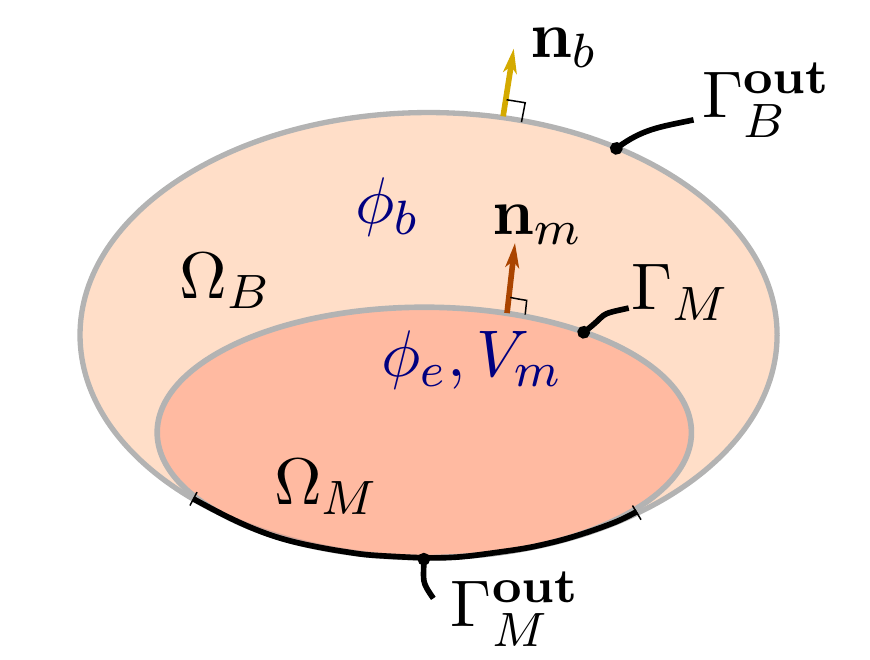
\includegraphics[width=50mm]{images/theory/computational_domains.png}
  \caption{Computational domains for the simulation of surface EMG. The body domain $\Omega_B$ and the muscle domain $\Omega_M$ share a part of their boundary, $\Gamma_M$, which has a normal vector $\bfn_m$. The outer boundary is composed of $\Gamma_B^\text{out}$ and $\Gamma_M^\text{out}$ and has the outward normal vector $\bfn_b$. }
  \label{fig:body_domain_visualization}
\end{figure}

The work of \cite{Mordhorst2015} proposes an isotropic conductivity $\bfsigma_b$ and a harmonic electric potential $\phi_b$ in the body domain $\Omega_B$:
\begin{align}\label{eq:body}
  \div \big(\bfsigma_b\,\grad (\phi_b)\big) = 0 \qquad \text{on } \Omega_B.
\end{align}

The electric potentials $\phi_e$ and $\phi_b$ of the neighboring domains $\Omega_M$ and $\Omega_B$ as well as the current densities are continuous on the shared boundary $\Gamma_M$. This is described by the following two coupling conditions:
\begin{subequations}\label{eq:body_domain_coupling}
  \begin{align}
    \phi_e &= \phi_b  \qquad &&\text{on } \Gamma_M, \label{eq:body_domain_bc1}   \\[4mm]
    \big(\bfsigma_e\, \grad( \phi_e)\big)\cdot \bfn_m &= \big(\bfsigma_b\, \grad(  \phi_b)\big)\cdot \bfn_m \qquad &&\text{on } \Gamma_M.\label{eq:body_domain_bc2}
  \end{align}
\end{subequations}
% 
On the outer boundary $\Gamma_B^\text{out}$, homogeneous Neumann boundary conditions are assumed:
\begin{align}
  \big(\bfsigma_b\, \grad( \phi_b)\big)\cdot \bfn_b &= 0 \qquad &&\text{on } \Gamma^\text{out}_B.\label{eq:body_domain_bc3}
\end{align}

The description of the body domain has to be combined either with the fiber based description in \cref{sec:monodomain_model} or the multi-domain description in \cref{sec:multidomain_model}. In the literature, this combination was mathematically described for the fiber based model in \cite{Mordhorst2015} and for the multidomain model in \cite{Klotz2020}. Correspondingly, additional boundary conditions either given by \cref{eq:monodomain_bc} or \cref{eq:multidomain_bc} are assumed: For the fiber based description, which uses the bidomain equation for volume conduction, the boundary conditions are:%
\begin{subequations}
\begin{align}
  \big(\bfsigma_i\,\grad(V_m)\big) \cdot \bfn_m &= -\big(\bfsigma_i\,\grad(\phi_e)\big)\cdot \bfn_m && \quad\text{on }∂\Omega_M=\Gamma_M \cup \Gamma_M^\text{out}, \label{eq:monodomain_fat_bc1}\\[4mm]
  \big(\bfsigma_e\,\grad(\phi_e)\big) \cdot \bfn_m &=0  && \quad\text{on }∂\Gamma_M^\text{out}. \label{eq:monodomain_fat_bc2}
\end{align}
\end{subequations}
%
For the multidomain description with fat layer, the boundary conditions are:
\begin{subequations}
\begin{align}
  \big(\bfsigma_i^k\,\grad(V_m^k)\big) \cdot \bfn_m &= -\big(\bfsigma_i^k\,\grad(\phi_e)\big)\cdot \bfn_m && \quad\text{on }∂\Omega_M=\Gamma_M \cup \Gamma_M^\text{out},  \label{eq:multidomain_fat_bc1}\\[4mm]
  \big(\bfsigma_e\,\grad(\phi_e)\big) \cdot \bfn_m &= 0 && \quad\text{on }∂\Gamma_M^\text{out}. \label{eq:multidomain_fat_bc2}
\end{align}
\end{subequations}
The first condition in \cref{eq:multidomain_fat_bc1} is enforced for all compartments $k=1,\dots,N_\text{MU}$.
%


% ----------
\subsection{Model of Muscle Contraction}\label{sec:model_muscle_contraction}

Muscle contraction is described on the organ level by a description of solid mechanics. Because of possibly large strains, a nonlinear hyperelastic formulation is used. For mathematical foundations in continuum mechanics, we refer to basic literature such as the books of Holzapfel \cite{holzapfel2000nonlinear} and Marsden and Hughes \cite{marsden1994mathematical}, as well as literature on the application of the Finite Element Method in continuum mechanics \cite{zienkiewicz1977finite,SUSSMAN1987357,zienkiewicz2005finite}.

% assumptions
We consider the 3D muscle domain $\Omega_0=\Omega_M \subset \R^3$ in reference configuration at time $t=0$ that deforms into a current configuration $\Omega_t$ at time $t$. The material points are given by $\bfX \in \Omega_0$. The corresponding points $\bfx \in \Omega_t$ in the current configuration are defined by the placement function $\bfx = \bfvarphi_t(\bfX)$. In the following, capital letters refer to quantities in material or Lagrangian description, i.e., defined in the reference configuration and small letters refer to quantities in spatial or Eulerian description, i.e., defined in the current configuration.

The relation of point coordinates in the current configuration with respect to the reference configuration can also be described by the displacements field $\bfu$:
\begin{align*}
  \bfx(\bfX) = \bfX + \bfu(\bfX).
\end{align*}
The current velocity $\bfv$ is the time derivative of the displacements, $\bfv := \dot{\bfu}$.

The foundation of continuum mechanics usually builds on three balance principles: conservation of mass, of momentum and of angular momentum. In the following, these principles are presented in their Eulerian forms.

First, we assume \emph{conservation of mass} in terms of the densities $\rho_0(\bfX)$ and $\rho(\bfx)$ in reference and current configurations:
%
\begin{align*}
  \ds\int\limits_{V_0} \rho_0\,\d V = \int\limits_{V_t} \rho \,\d v.
\end{align*}
%
The equation holds for all corresponding subdomains $V_0\subset \Omega_0$ and $V_t \subset \Omega_t$. With the intermediate step of deducing $\d/\d t \int_{\Omega_t} \rho \,\d v=0$, we get the following differential equation:%
\begin{align}\label{eq:contraction_helper1}
  \dot{\rho}(\bfv,t) + \rho(\bfx,t)\,\div\big(\bfv(\bfx,t)\big) = 0.
\end{align}
%

As muscle tissue largely consists of water, it is typically assumed to be an incompressible domain. This is equivalent to a constant density, $\dot{\rho}=0$, and, thus, \cref{eq:contraction_helper1} reduces to
%
\begin{align}\label{eq:assumption_1_local}
  \div(\bfv(\bfx,t)) = 0.
\end{align}
%

The second assumption is the \emph{balance of momentum}, which is expressed as %
\begin{align*}
  \d{t} \ds\int\limits_{V_t} \rho\,\bfv\, \d v = \ds\int\limits_{V_t} \rho\,\bfb \,\d v + \ds\int\limits_{∂V_t} \bft \,\d a.
\end{align*}
Here, $\bfb$ describes a body force and $\bft$ describes a traction force that acts on the surface of the current configuration. The corresponding differential form is given by the following differential equation:%
\begin{align}\label{eq:assumption_2_local}
  \rho\,\dot{\bfv}(\bfx,t) = \rho\,\bfb(\bfx,t) + \div\bfsigma(\bfx,t).
\end{align}
%
The second order Cauchy stress tensor $\bfsigma$ has units of force per area and is defined by the relation $\bft = \bfsigma \bfn$ between a traction force $\bft$ in a virtual cut out of the body at $\bfx$ and the normal vector $\bfn$ of the cut area.

The third assumption is the \emph{balance of angular momentum} and can be formulated using the 3D cross-product:%
\begin{align*}
  \d{t} \ds\int\limits_{V_t} \bfx \times (\rho\,\bfv)\, \d v = \ds\int\limits_{V_t} \bfx \times (\rho\,\bfb) \,\d v + \ds\int\limits_{∂V_t} \bfx \times \bft\,\d a.
\end{align*}
%
Derivations yield equivalence to the symmetry of the Cauchy stress tensor, $\bfsigma = \bfsigma^\top$.

A further assumption in the multi-scale muscle framework is to only consider isothermal conditions. 
An activated muscle performs work and by metabolism energy is added to the system. Further, the muscle is not thermodynamically isolated. The system is not closed regarding conversion and transfer of energy and, thus, the balance of energy cannot be modeled easily.

The mathematical description has to be closed by defining a constitutive relation between stresses and strains. The usual approach for hyperelastic materials is to define a strain energy function $\Psi$. This scalar function is formulated in terms of the right Cauchy-Green tensor $\bfC$, which is related to the strain of the deformed body. Then, the stresses are given by%
\begin{align*}
  \bfS = 2\p{\Psi(\bfC)}{\bfC},
\end{align*}
where $\bfS$ is the second Piola-Kirchhoff stress tensor, which in the incompressible case is the pull-back of the Cauchy stress $\bfsigma$ used in the balance of momentum in \cref{eq:assumption_2_local}.
%which is related to the Cauchy stress $\bfsigma$ used in the balance of momentum in \cref{eq:assumption_2_local}.

%It is usually formulated in terms of the five principle strain invariants $I_1$ to $I_5$. A derivative of $\Psi$ is used to derive a term for the stress. More details follow in \cref{sec:discretization_mechanics}.

In the muscle contraction model of \cite{Heidlauf2013}, the strain energy function is additively composed of two passive terms, one isotropic and one anisotropic, and one additional active term:
\begin{align*}
  \Psi(\bfC) = \Psi_\text{isotropic}(I_1,I_2) + \Psi_\text{anisotropic}(\lambda_f) + \Psi_\text{active}(\gamma).
\end{align*}
The isotropic term $\Psi_\text{isotropic}$ is formulated in terms of the strain invariants $I_1=\tr(\bfC)$ and $I_2=\big(\tr(\bfC)^2 - \tr(\bfC^2)\big)/2$. The anisotropic term $\Psi_\text{anisotropic}$ depends on the fiber stretch $\lambda_f$. The active term $\Psi_\text{active}$ yields the active stress that results from muscular activation, which is described by the activation parameter $\gamma$.
%Note the missing dependency on the third invariant $I_3$, which is constant because of the enforced incompressibility.

The passive behavior of muscle tissue is modeled by a transversely isotropic Mooney-Rivlin material.
The isotropic part is given by the Mooney-Rivlin formulation:%
\begin{align}\label{eq:mooney_rivlin}
  \Psi_\text{isotropic}(I_1,I_2) = c_1\,(I_1 - 3) + c_2\,(I_2-3).
\end{align}
The values of the two material parameters $c_1$ and $c_2$ can be determined by compression tests and are summarized in the work of \cite{Heidlauf2013}.

The anisotropic behavior depends only on the fiber stretch $\lambda_f$. The formulation in \cite{Heidlauf2013} uses two material parameters $b$ and $d$ and the following function:
\begin{align*}
  \Psi_\text{anisotropic}(\lambda_f) = \dfrac{b}{d}(\lambda_f^d - 1) - b\,\log(\lambda_f).
\end{align*}
%

The active contribution is directly formulated in terms of the second Piola-Kirchhoff stress $\bfS$. The relation between the active stress $\bfS_\text{active}$ and the active contribution $\Psi_\text{active}$ of the strain energy function as well as the definition of $\bfS_\text{active}$ are given as follows:
\begin{align}\label{eq:active_stress_term}
  \bfS_\text{active} = \dfrac{1}{\lambda_f}\p{\Psi_\text{active}}{\lambda_f} \bfA \otimes \bfA = \dfrac{1}{\lambda_f} \cdot S_\text{max,active}\cdot f_\ell(\lambda_f)\cdot\bar{\gamma}\, \bfA \otimes \bfA,
\end{align}
%
Here, the resulting active stress tensor $\bfS_\text{active}$ is the second order tensor oriented according to the material fiber direction $\bfA: \Omega_0 \to \R^3$ and given by the dyadic product $\bfA \otimes \bfA = A_{i}\,A_{j}\,\bfe_i \otimes \bfe_j$, scaled by the maximum active stress parameter $S_\text{max,active}$, a function $f_\ell$ that models the force-length relation, and the 3D homogenized value $\bar{\gamma}$ of the activation parameter $\gamma \in [0,1]$ following from the half-sarcomere model.

In the deforming body fat layer, the active stress contribution is disregarded. For simulating tendons, different material models can be used such as the model proposed by Carniel et al. \cite{Carniel2017}, which describes microstructural interactions between collagen fibers and their matrix in addition to the elastic response of the fibers itself. To alter the material model, the definition of $\Psi$ can simply be changed while all other equations remain intact. Similarly, other material models can be defined using the framework of the strain energy function.

In short summary, the following system of equations describes the continuum mechanics model of muscle contraction:
%
\begin{subequations}\label{eq:contraction}
  \begin{align}
    \div(\bfv) &= 0, \qquad &&\text{(incompressibility)} \label{eq:contraction_1}\\[4mm]
    \rho\,\dot{\bfv} &= \rho\,\bfb + \div\bfsigma, && \text{(balance of linear momentum)}\label{eq:contraction_2}\\[4mm]
    \bfsigma &= \bfsigma^\top, && \text{(balance of angular momentum)}\label{eq:contraction_3}\\[4mm]
    \bfS &= 2\p{\Psi(\bfC)}{\bfC}, && \text{(constitutive equation)}\label{eq:contraction_4}
  \end{align}
\end{subequations}
with a material model that defines the strain energy function $\Psi$.

Dirichlet boundary conditions for the displacements $\bfu$ and velocities $\bfv$ can fix certain parts of the muscle, e.g., at the attachment points of the tendons:
\begin{align*}
  \bfu(\bfx,t) &= \bar{\bfu}(t), & \bfv(\bfx,t) &= \bar{\bfv}(t) \quad &&\text{for } \bfx \in ∂\Omega_\text{Dirichlet}.
\end{align*}
%
Initial conditions for $\bfu$ and $\bfv$ define the initial pose of the muscle tissue:
%
\begin{align*}
  \bfu(\bfx,0) &= \bfu_0(\bfx), & \bfv(\bfx,0) &= \bfv_0(\bfx) \quad &&\text{for } \bfx \in \Omega_M.
\end{align*}
%
Additionally, Neumann boundary conditions can be used to prescribe traction forces on the surface.

The description of the multi-scale model \cite{Roehrle2012,Heidlauf2013} assumes quasi-static conditions, which means that the velocities are set to zero, $\bfv=\bfzero$, and inertial terms are neglected. In consequence, the incompressibility constraint in \cref{eq:contraction_1} has to be formulated differently and the balance of momentum in \cref{eq:contraction_2} reduces to $\rho\,\bfb + \div \bfsigma = 0$.
However, our implementation extends the model to the fully dynamic formulation given in \cref{eq:contraction_1,eq:contraction_2,eq:contraction_3,eq:contraction_4}. 

More details on the mechanics equations, their discretization and the resulting numerical scheme to obtain the solution functions $\bfu$ and $\bfv$ are given in \cref{sec:discretization_mechanics}.


%\subsection{Sensory Organs and Motor Neurons}
%text of paper:
%Muscle spindles and Golgi tendon organs are located in the muscle and sense fiber stretch, contraction velocity, contraction acceleration and muscle forces. 
%They are connected via layers of inter neurons to the motor neurons, which reside in the spinal cord.
%In turn, the motor units innervate and activate the muscle.

%We use CellML models to compute the dynamics of muscle spindles \cite{Mileusnic2006} and motor neurons \cite{CisiKohn2008}.

\section{Discretization}\label{sec:discretization}

The partial and ordinary differential equations described in the last section contain spatial an temporal derivatives that have to be discretized to be numerically solved. For temporal derivatives, we use timestepping schemes, for spatial derivatives, we employ the Finite Element Method.

In this section, we describe the discretization of the subcellular and electrophysiology models that were presented in the last section. A description of the discretization of the solid mechanics model follows in \cref{sec:discretization_mechanics}.

We begin with the discretization in time in \cref{sec:discretization_monodomain}, followed by the spatial discretization for the monodomain (\cref{sec:discretization_diffusion,sec:mass_lumping}) and multidomain models (\cref{sec:discretization_multidomain,sec:discretization_body_domain}).

\subsection{Discretization of the Monodomain Model}\label{sec:discretization_monodomain}

Electrophysiology models typically consists of a reaction-diffusion equation. The diffusion term describes the electric conduction in the tissue and the reaction term includes the subcellular model. In our model, the monodomain equation used in the fiber based description, \cref{eq:monodomain}, and the second multidomain equation, \cref{eq:multidomain2}, are equations of this type.

This type of partial differential equation is often solved using operator splitting schemes. A first order operator splitting scheme is Godunov splitting \cite{Godunov2003}. It was used for the solution of the chemo-electro-mechanical model in \cite{Roehrle2012}. In addition to Godunov splitting, we also employ the second order accurate Strang splitting scheme \cite{Strang1968}.

In the following, the application of these two schemes is illustrated with the monodomain equation, \cref{eq:monodomain}. The right hand sides of the diffusion and reaction terms are designated as $\mathcal{L}_1$ and $\mathcal{L}_2$:%
\begin{align*}
  \mathcal{L}_1(V_m) := \dfrac{1}{A_m\,C_m} \sigma_\text{eff}\dfrac{\partial^2 V_m}{\partial x^2}, &&
  \mathcal{L}_2(V_m) := -\dfrac{1}{C_m} I_\text{ion}(V_m,\bfy).
\end{align*}
%
Then, the monodomain equation takes the form:
%
\begin{align*}
  \p{V_m}{t} = \mathcal{L}_1(V_m) + \mathcal{L}_2(V_m).
\end{align*}

A timestepping scheme is constructed that starts with a given initial value $V_m^{(0)}$ and computes solution values $V_m^{(i)}$ at discrete points in time $t^{(i)} = i\cdot\dt$ with a fixed timestep width $\dt$.
Godunov splitting proceeds by alternatingly solving the ODEs with right hand sides $\mathcal{L}_1$ and $\mathcal{L}_2$. In the first substep per iteration, an intermediate value $V_m^{\ast}$ is calculated, which is used as starting point for the second substep. Each of the substeps are performed using another timestepping scheme for the ODE, e.g., the explicit Euler scheme:
%
\begin{subequations}\label{eq:monodomain_godunov}
  \begin{align}
    V_m^{\ast} &= V_m^{(i)} + \dt \mathcal{L}_1(V_m^{(i)},t^{(i)}),\\[4mm]
    V_m^{(i+1)} &= V_m^{\ast} + \dt \mathcal{L}_2(V_m^{\ast},t^{(i)})
  \end{align}
\end{subequations}

Strang splitting uses a similar approach with three substeps per timestep and two intermediate values $V_m^{\ast}$ and $V_m^{\ast\ast}$:
%
\begin{subequations}\label{eq:monodomain_strang}
  \begin{align}
    V_m^{\ast} &= V_m^{(i)} + \dfrac{\dt}{2} \mathcal{L}_1(V_m^{(i)},t^{(i)}),\\[4mm]
    V_m^{\ast\ast} &= V_m^{\ast} + \dt \mathcal{L}_2(V_m^{\ast},t^{(i)}),\\[4mm]
    V_m^{(i+1)} &= V_m^{\ast\ast} + \dfrac{\dt}{2} \mathcal{L}_1(V_m^{\ast\ast},t_{(i)}+\dfrac12 \dt).
  \end{align}
\end{subequations}
%
% stuff needed to create the plot
%\definecolor{vred}{RGB}{170,0,0}
%\definecolor{vyellow}{RGB}{212,170,0}
%\definecolor{vgreen}{RGB}{0,170,0}
%\begin{equation*}
%  \begin{array}{lll}
%    \frac{\partial}{\partial t} V_m  = \textcolor{vred}{c_1 \frac{\partial^2}{\partial x^2} V_m }\\[4mm]
%    \frac{\partial}{\partial t} \bfy = \textcolor{vyellow}{G(V_m,\bfy)}\\[4mm]
%    \frac{\partial}{\partial t} V_m = \textcolor{vyellow}{c_2\,I_\text{ion}(V_m,\bfy)}\\[4mm]
%    \textcolor{vyellow}{\dt_\text{0D}}\quad
%    \textcolor{vred}{\dt_\text{1D}}\quad
%    \dt_\text{splitting}\quad
%    \textcolor{vgreen}{\dt_\text{3D}}\quad
%    t^{(i)}, t^{(i)} + \dt_\text{splitting}/2, t^{(i)} + \dt_\text{splitting} ...\\[4mm]
%    t^{(i)} + \textcolor{vgreen}{\dt_\text{3D}}\\[4mm]
%    t^{(i+1)}
%  \end{array}
%\end{equation*}
%\textcolor{vyellow}{0D:}
%\textcolor{vred}{1D:}
%\textcolor{vgreen}{3D:}

\Cref{fig:splitting_schemes} visualizes both splitting schemes applied to the monodomain equation. 
The yellow arrows correspond to the solution of the 0D subcellular model. The red arrows correspond to the solution of the 1D diffusion equation. The timestepping schemes of the substeps have timestep widths $\dt_\text{0D}$ and $\dt_\text{1D}$, respectively. The timestep width of one splitting step is $\dt_\text{splitting}$. Depending on how the timestep widths are chosen in relation to each other, different numbers of subcycles are used in the solution of the 0D and 1D problems.

\begin{figure}%
  \centering%
  \begin{subfigure}[t]{0.48\textwidth}%
    \centering%
    \def\svgwidth{\textwidth}
    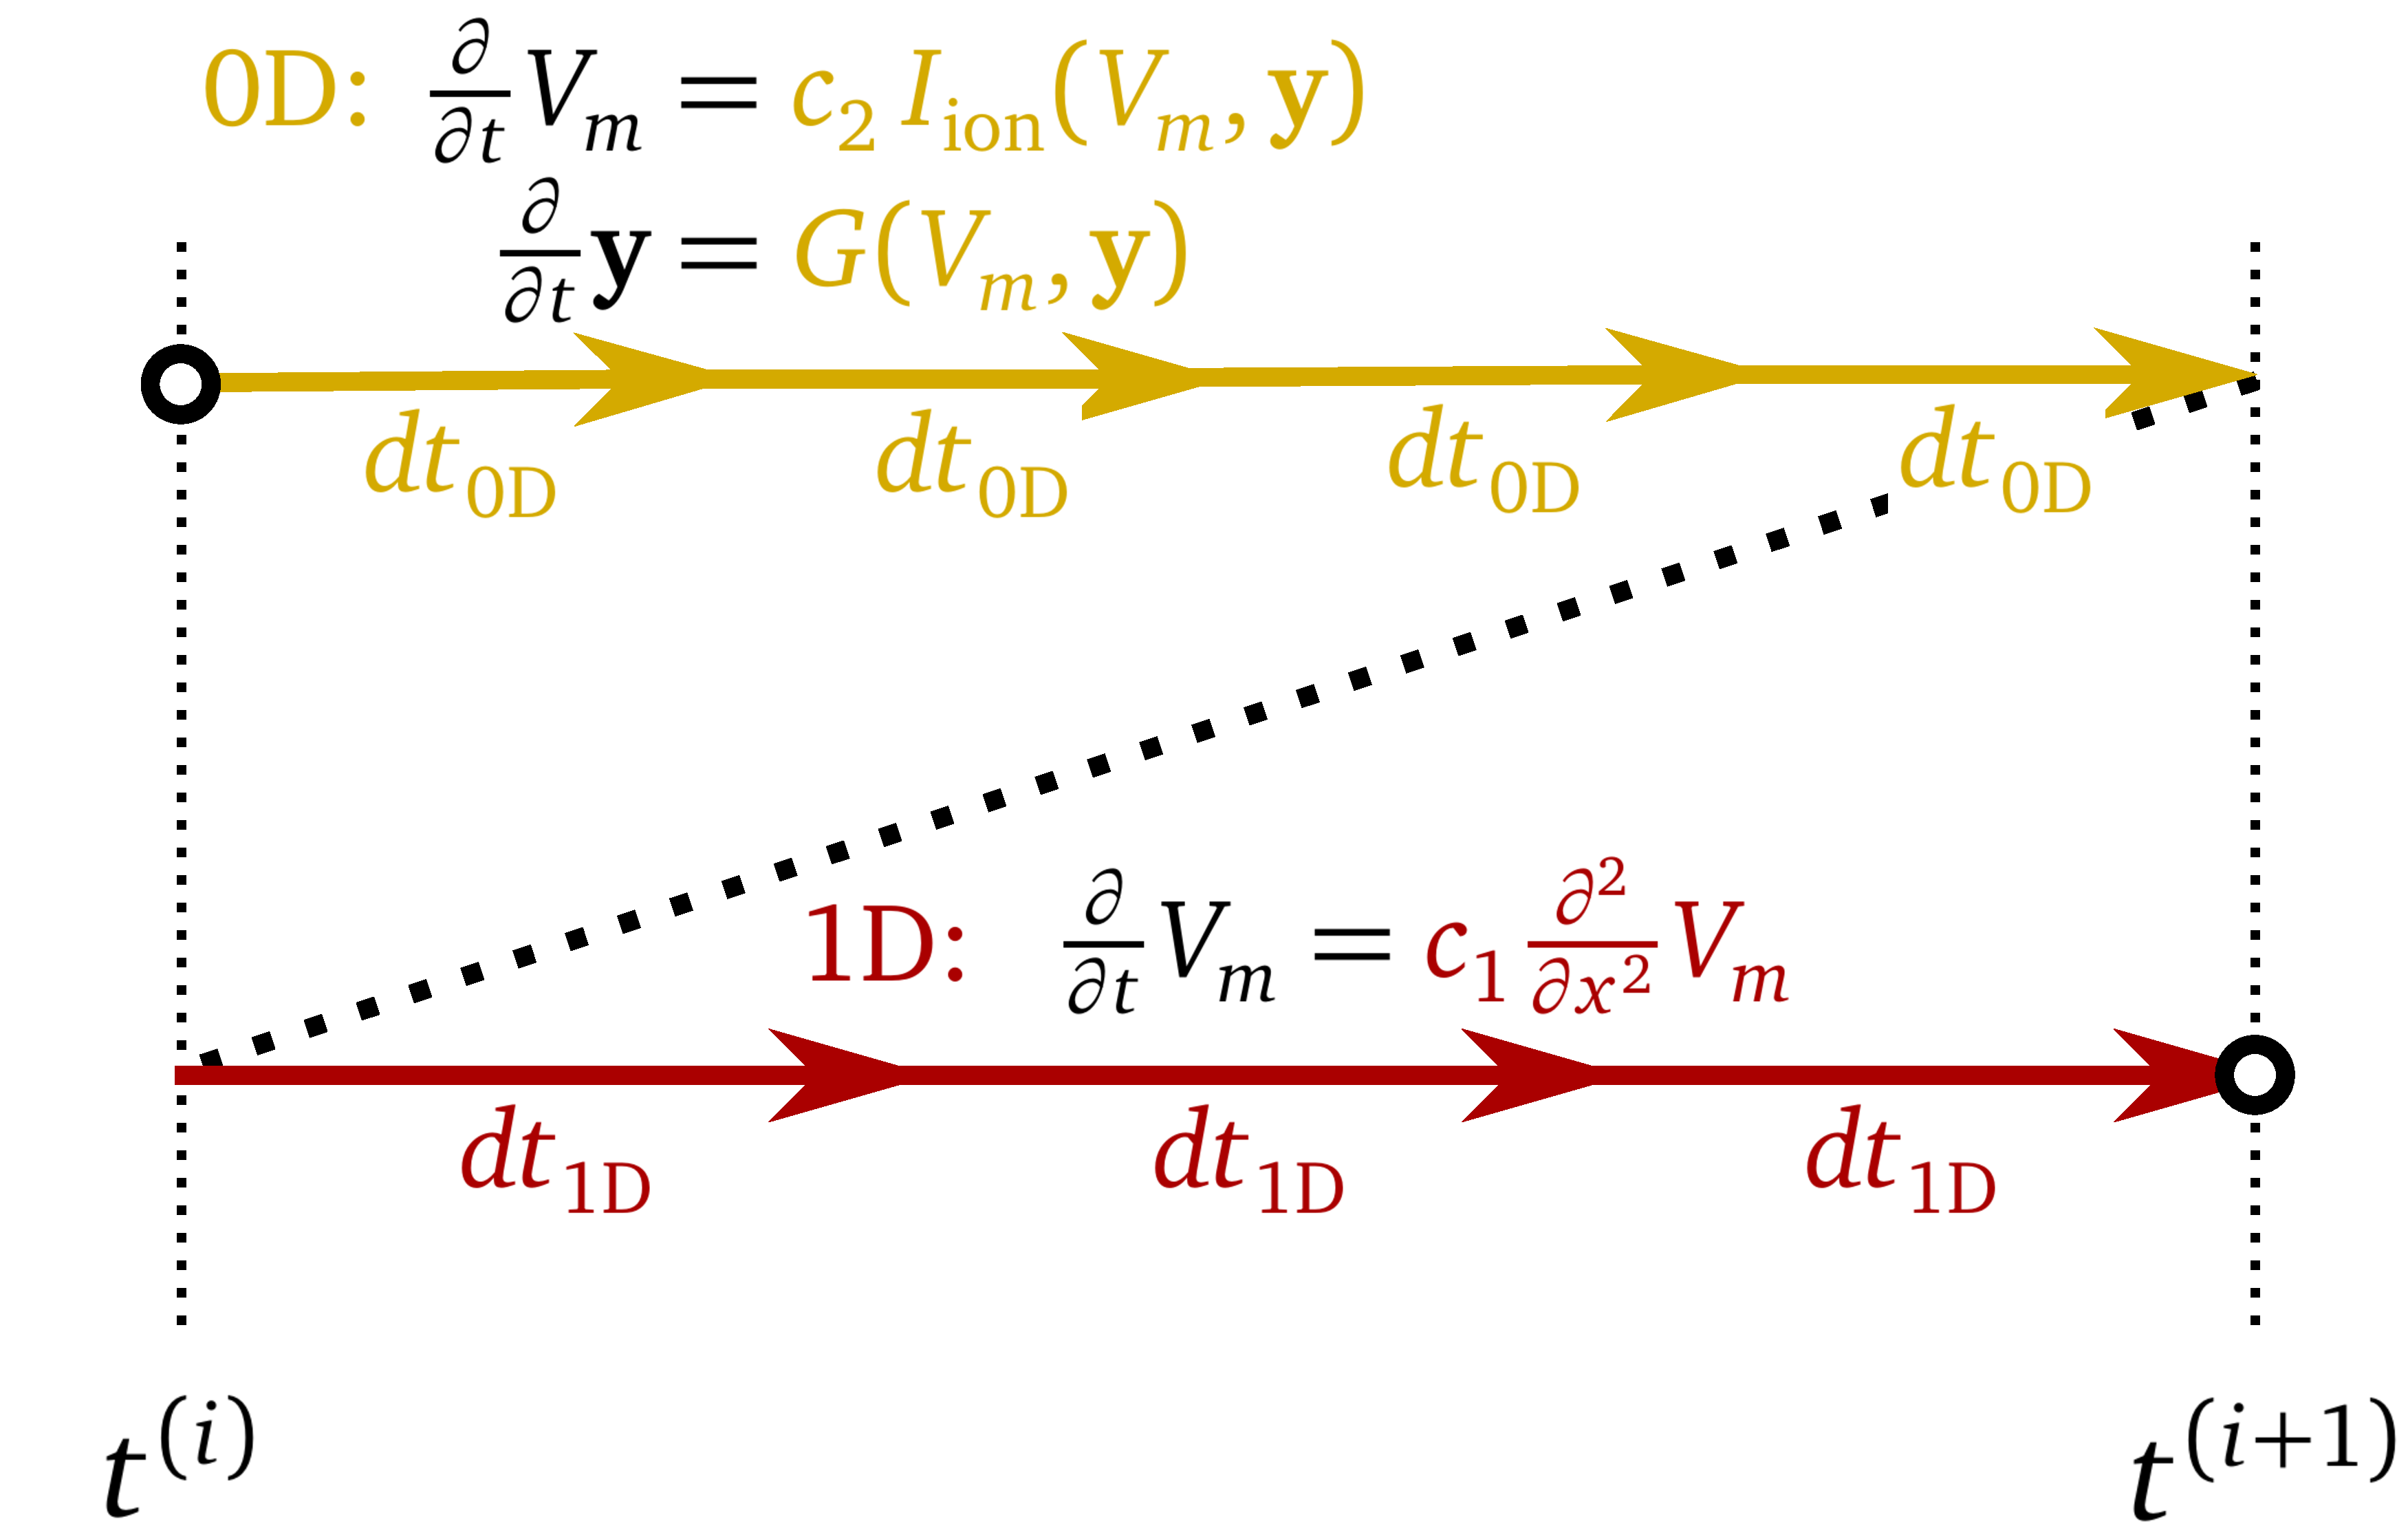
\includegraphics[width=\textwidth]{images/theory/godunov_splitting.pdf}
    \caption{The Godunov splitting uses two substeps: 0D, 1D.}%
    \label{fig:godunov_splitting}%
  \end{subfigure}
  \quad
  \begin{subfigure}[t]{0.48\textwidth}%
    \centering%
    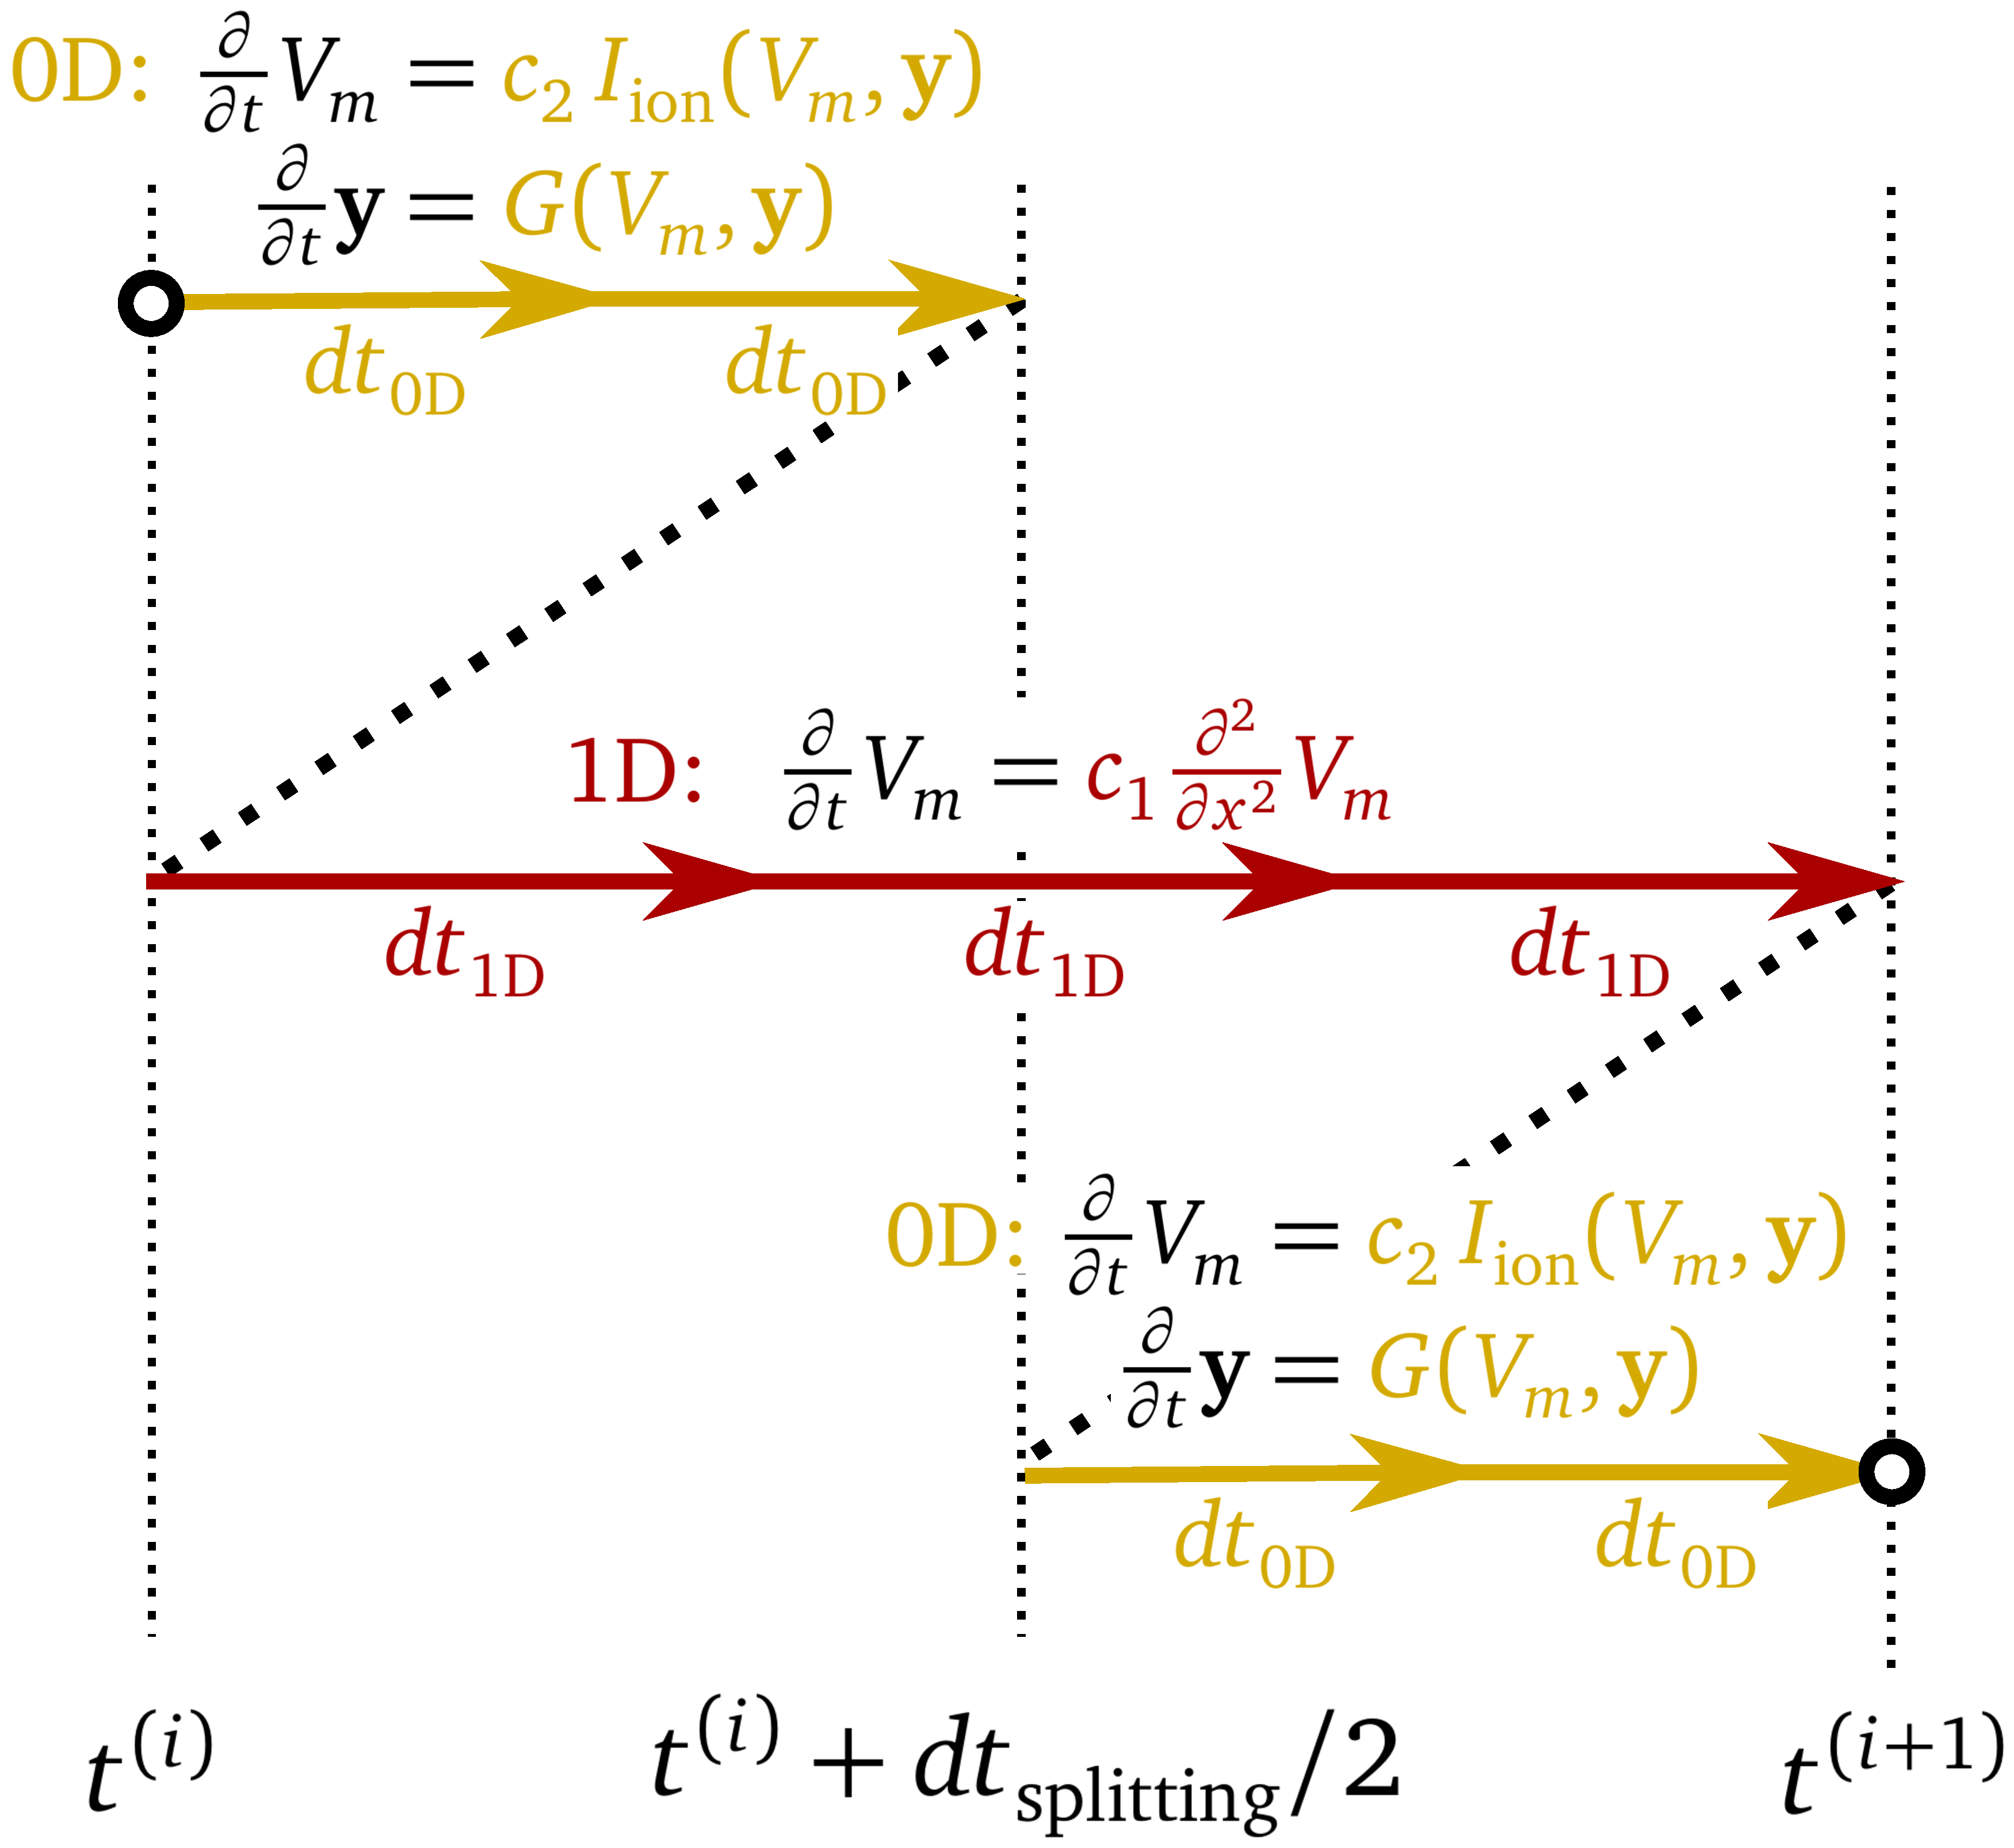
\includegraphics[width=\textwidth]{images/theory/strang_splitting.pdf}
    \caption{The Strang splitting uses three substeps: 0D, 1D, 0D.}%
    \label{fig:strang_splitting}%
  \end{subfigure}
  \caption{Godunov and Strang splitting schemes that are used to solve the monodomain equation. The equation is split into a reaction part (0D,yellow) and a diffusion part (1D,red) and these parts are solved alternatingly. The visualizations show one splitting timestep starting at the left circle and completing at the right circle.}%
  \label{fig:splitting_schemes}%
\end{figure}%

Instead of the explicit Euler method in \cref{eq:monodomain_godunov,eq:monodomain_strang}, other timestepping methods can be used for the substeps. 
We use the following schemes, which are listed as single iteration step for the generic ODE ${\p V_m / \p t = \mathcal{L}(V_m,t)}$:
\begin{subequations}\label{eq:ode_solver_schemes}
  \begin{align}
    V_m^{(i+1)} &= V_m^{(i)} + \dt \mathcal{L}(V_m^{(i)},t^{(i)}), \label{eq:explicit_euler}\\[4mm]
    V_m^{(i+1)} &= V_m^{(i)} + \dfrac{\dt}{2}\Big(
      \mathcal{L}(V_m^{(i)},t^{(i)}) + \mathcal{L}\big(V_m^{(i)} + \dt \mathcal{L}(V_m^{(i)},t^{(i)}),t^{(i+1)}\big)\Big), \label{eq:heun}\\[4mm]
    V_m^{(i+1)} &= V_m^{(i)} + \dt \mathcal{L}(V_m^{(i+1)},t^{(i+1)}), \label{eq:implicit_euler}\\[4mm]
    V_m^{(i+1)} &= V_m^{(i)} + \dfrac{\dt}{2}\Big(
      \theta\,\mathcal{L}(V_m^{(i+1)},t^{(i+1)}) + (1-\theta)\,\mathcal{L}(V_m^{(i)},t^{(i)})\Big).\label{eq:crank_nicolson}
  \end{align}
\end{subequations}
%
Here, \cref{eq:explicit_euler} is the first-order accurate explicit Euler scheme, \cref{eq:heun} is the second-order accurate Heun scheme, \cref{eq:implicit_euler} is the first order accurate implicit Euler scheme and \cref{eq:crank_nicolson} is the Crank-Nicolson scheme \cite{CrankNicolson1947}, which for $\theta=0$ equals the explicit Euler and for $\theta=1$ equals the implicit Euler scheme. For $\theta=\frac12$, it is second order accurate. An advantage of the implicit schemes in \cref{eq:implicit_euler,eq:crank_nicolson} is that, for our considered diffusion problems, they are unconditionally stable. A disadvantage is that a linear equation has to be solved in every timestep.

A second order accurate timestepping scheme allows a higher timestep width to yield the same numerical error as a first order scheme.
To obtain a second order scheme for the monodomain equation, we use Strang splitting (\cref{eq:monodomain_strang}) with the Crank-Nicolson scheme (\cref{eq:crank_nicolson}) for the diffusion term $\mathcal{L}_1$ and Heun's method (\cref{eq:heun}) for the reaction term $\mathcal{L}_2$. In the subcellular model, the system of ODEs with state vector $\bfy$ given in \cref{eq:subcellular} is solved with Heun's method along with the equation in terms of $V_m$.

Next, the spatial derivatives in the diffusion part $\mathcal{L}_2$ of the split equation have to be discretized. Then, both the multidomain and the fiber based models can be solved using the splitting scheme.

\subsection{Discretization of the Diffusion and Laplace Equations}\label{sec:discretization_diffusion}

For the spatial discretization, we first derive the Finite Element formulation for a generic parabolic diffusion equation in a domain $\Omega\subset\R^d$ of arbitrary dimensionality $d$. Then, specialization to 1D yields the formulation for the monodomain equation. Considering a 3D domain, the formulation is an important building block for the discretization of the multidomain model. This is shown in more detail in a later section, \cref{sec:discretization_multidomain}

We consider the following diffusion problem in the variable $u: \Omega \times [0,t_\text{end}] \to \R$ with Neumann boundary conditions on a part of the boundary $\Gamma_f \subset ∂\Omega$ with normal vector $\bfn$:
\begin{align*}
  \p{u}{t} &= \div(\bfsigma \grad u), &(\bfsigma\,\grad u) \cdot \bfn &= f \quad \text{on }\Gamma_f, & (\bfsigma\,\grad u) \cdot \bfn &= 0 \quad \text{on } ∂Ω\backslash \Gamma_f.
\end{align*}
We discretize the temporal derivative using the Crank-Nicolson scheme of \cref{eq:crank_nicolson}. Following the procedure of the Galerkin Finite Element formulation with the Hilbert space $H^1_0(\Omega)$ of test functions $\phi$ that are zero on the boundary, we arrive at the following weak form:
%
\begin{align*}
  \ds\int_Ω \big(\theta\,∇\cdot(\bfsigma ∇ \bfu^{(i+1)})  + (1-\theta)\,∇\cdot(\bfsigma ∇ u^{(i)})\big)\,\phi \,\d\bfx &&\\
    \qquad = \dfrac{1}{\dt} \ds\int_Ω(u^{(i+1)} - u^{(i)})\,\phi\,\d\bfx, &&\qquad \forall \phi \in H^1_0(\Omega).
\end{align*}
For brevity, we express divergence and gradient using the nabla operator. 

To discretize the weak form, we choose a function space $V_h = \text{span}\{\varphi_j \mid j = 1, \dots, N\}$ to represent the solution as $u = \sum_{j=1}^N u_j \phi_j$. Applying the divergence theorem, we obtain:
\begin{equation}\label{eq:diffusion_helper1}
  \begin{array}{l}
    \ds\sum\limits_{j=1}^{N} \big(\theta\,u_j^{(i+1)} + (1-\theta)\,u_j^{(i)}\big)  
    \left(-\ds\int_Ω \bfsigma\,∇\varphi_j\cdot ∇\varphi_k \,\d\bfx + \ds\int_{∂Ω} \big(\bfsigma\,∇\varphi_j\cdot \bfn\big)\,\varphi_k \,\d\bfx  \right) \\
      \quad = \dfrac{1}{\dt} \sum\limits_{j=1}^{N} \big(u_j^{(i+1)} - u_j^{(i)}\big) \ds\int_Ω \varphi_j\,\varphi_k\,\d\bfx, \qquad \forall k = 1,\dots, N.
  \end{array}
\end{equation}
This iteration step can be written in matrix notation in terms of the vectors of unknowns $\bfu^{(i)}=(u^{(i)}_0,\dots,u^{(i)}_N)^\top$ at timestep $i$:%
\begin{align*}
  \bfA\,\bfu^{(i+1)} = \bfb(\bfu^{(i)}).
\end{align*}
The system matrix $\bfA$ and the right hand side $\bfb$ are given by:
\begin{align*}
  \bfA &= \theta\,(\bfK_{\bfsigma} + \bfB_{\bfsigma}) -\dfrac{1}{\dt}\bfM, &
  \bfb &= \big((\theta-1)\,(\bfK_{\bfsigma} + \bfB_{\bfsigma}) - \dfrac{1}{\dt} \bfM \big)\,\bfu^{(i)}.
\end{align*}
The formulation uses the standard stiffness matrix $\bfK_{\bfsigma}$, the matrix $\bfB_{\bfsigma}$ of the boundary integral and the mass matrix $\bfM$, whose components are defined as%
\begin{align}\label{eq:diffusion_matrices}
  \bfK_{\bfsigma,kj} &= -\ds\int_Ω (\bfsigma\, ∇\varphi_j)\cdot ∇\varphi_k \,\d\bfx,&
     \bfB_{\bfsigma,kj} &= \ds\int_{\Gamma_f} \big((\bfsigma\,∇\varphi_j)\cdot \bfn\big)\,\varphi_k \,\d\bfx,&
     \bfM_{kj} &= \ds\int_Ω \varphi_j\,\varphi_k\,\d\bfx.
\end{align}
Note that after applying the divergence theorem, the definition of the stiffness matrix has a minus sign, which is correct for the positive second order derivative in the original diffusion term.

Next, we take into account the Neumann boundary condition $\bfsigma∇u\cdot \bfn = f$ on the boundary $\Gamma_f$. The flux $f$ over the boundary is discretized by $M$ separate ansatz functions $\psi_j$ on $\Gamma_f$ as $f = \sum_{j=1}^M f_j\, \psi_j$.
The flux values are summarized in a vector $\bff=(f_1,\dots,f_M)^\top$.
Plugging this into \cref{eq:diffusion_helper1} yields the following equation in matrix notation:%
\begin{align}\label{eq:diffusion_helper2}
  \tilde{\bfA}\,\bfu^{(i+1)} = \tilde{\bfb}(\bfu^{(i)}),  
\end{align}
with the system matrix $\tilde{\bfA}$ and right hand side $\tilde{\bfb}$: 
\begin{align*}
  \tilde{\bfA} &= \theta\,\bfK_{\bfsigma} -\dfrac{1}{\dt}\bfM, &
    \tilde{\bfb} &= \big((\theta-1)\,\bfK_{\bfsigma} - \dfrac{1}{\dt} \bfM \big)\,\bfu^{(i)} - \bfB_{\Gamma_f}\,\big(\theta\,\bff^{(i+1)} + (1-\theta)\,\bff^{(i)}\big),
\end{align*}
and the boundary matrix $\bfB_{\Gamma_f}$ given by:
\begin{align}\label{eq:definition_boundary_matrix}
  \bfB_{\Gamma_f,kj} &= \ds\int_{\Gamma_f} \psi_j\,\varphi_k \,\d\bfx.
\end{align}
Note, incorporating the Neumann boundary conditions in the weak form corresponds to the following exchange of the boundary matrices $\bfB_\sigma$ and $\bfB_{\Gamma_f}$:%
\begin{align}\label{eq:boundary_relation}
  \bfB_\sigma\,\bfu = \bfB_{\Gamma_f}\,\bff.
\end{align}
%


\Cref{eq:diffusion_helper2} is used to solve the diffusion part of the monodomain equation given in \cref{eq:monodomain} after inserting the corresponding constant prefactors.

When deriving or implementing new models or optimizing solver code, it is often beneficial to study certain effects in isolation. It can help to use a toy problem such as the simple Laplace problem $Δu = 0$, possibly with Neumann boundary condition $\partial u/\partial \bfn = f$. 
By specializing the formulation in \cref{eq:diffusion_helper2} accordingly, we obtain the system
%
\begin{align*}
  (\bfK_\bfI + \bfB_\bfI)\,\bfu = \bfzero
\end{align*}
for the case without boundary condition (set $\bfB_\bfI$ to zero to assume homogenous Neumann boundaries) or
\begin{align}\label{eq:discretization_laplace}
  \bfK_\bfI\,\bfu = -\bfB_{\Gamma_f}\,\bff
\end{align}
to include the formulated Neumann boundary condition.

\subsection{Using Mass Lumping for Implicit Timestepping}\label{sec:mass_lumping}
Implicit timestepping schemes such as implicit Euler or the Crank-Nicoloson scheme for $\theta=\frac12$ need to solve a linear equation in every timestep.
Assuming homogeneous Neumann boundary conditions for simplicity, the iteration step of the canonical Crank-Nicolson scheme follows from \cref{eq:diffusion_helper2}:
\begin{subequations}\label{eq:lumping_crank_nicolson}
  \begin{align}
    \big(\dfrac1{2}\bfK-\dfrac{1}{\dt}\bfM\big)\, \bfu^{(t+1)} &= \big(-\dfrac12{\bfK} - \dfrac{1}{\dt}\bfM\big)\, \bfu^{(t)}\label{eq:lumping_crank_nicolson_1}\\[4mm]
    \Leftrightarrow \quad (\bfI - \dfrac{\dt}{2}\,\bfM^{-1}\bfK)\,\bfu^{(t+1)}&= \,\bfu^{(t)}(\bfI + \dfrac{\dt}{2}\,\bfM^{-1}\bfK).\label{eq:lumping_crank_nicolson_2}
  \end{align}
\end{subequations}
For the implicit Euler method, we obtain:%
\begin{subequations}\label{eq:lumping_implicit_euler}
  \begin{align}
    \ds(\bfK-\frac{\bfM}{\dt})\,\bfu^{(t+1)} &=\,\ds -\frac{\bfM}{\dt}\bfu^{(t)}\label{eq:lumping_implicit_euler_1}\\[4mm]
    \Leftrightarrow \quad (\bfI - \dt\,\bfM^{-1}\bfK)\,\bfu^{(t+1)}&= \,\bfu^{(t)}.\label{eq:lumping_implicit_euler_2}
  \end{align}
\end{subequations}
Both iteration steps in \cref{eq:lumping_crank_nicolson_1,eq:lumping_crank_nicolson_2} and in \cref{eq:lumping_implicit_euler_1,eq:lumping_implicit_euler} are equivalent, as the second equation follows from the first one by left multiplication of $(-\dt \bfM^{-1})$. In the second equations, the matrices to be multiplied are created by a sum of the unity matrix $\bfI$ and another matrix term that is scaled by the potentially small timestep width $\dt$. For the implicit Euler in \cref{eq:lumping_implicit_euler_2}, the matrix on the right hand side even completely vanishes. This is preferred over the first iteration steps in \cref{eq:lumping_crank_nicolson_1,eq:lumping_implicit_euler_1} as it leads to better conditioned matrix-vector multiplications.

The required inversions of the mass matrix cannot be carried out explicitly as the inversion would fill in numerous matrix entries and eliminate the sparse structure. This is not feasible for highly resolved meshes with a large number of degrees of freedom. Instead, \emph{mass lumping} is used, where the mass matrix $\bfM$ is approximated by a diagonal matrix with diagonal entries equal to the row sums in $\bfM$ \cite{Hinton1976}. Thus, multiplication with the inverse mass matrix corresponds to a rescaling of columns by the inverse lumped diagonal entries.

\subsection{Discretization of the Multidomain Model}\label{sec:discretization_multidomain}
With the prerequisites of temporal discretization in \cref{sec:discretization_monodomain} and the Finite Element formulation of a diffusion equation in \cref{sec:discretization_diffusion}, we can now discretize the multidomain model. Since this has not been previously done in literature using the Finite Element Method, the subsequent derivation is more detailed.

The first multidomain equation given in \cref{eq:multidomain1} yields the following form after applying the Finite Element derivation in \cref{eq:diffusion_helper2}:
%
\begin{align}\label{eq:multidomain_discretization_helper_multidomain1}
  \big(\bfK_{\bfsigma_e + \bfsigma_i} + \bfB_{\bfsigma_e + \bfsigma_i}\big)\,\bfphi_{e} +  \s{k=1}{N_\text{MU}} f_r^k \big(\bfK_{\bfsigma_i^k} + \bfB_{\bfsigma_i^k}\big)\,\bfV_m^k = 0.  
\end{align}
Here, $\bfphi_{e}$ and $\bfV_m^k$ are the vectors of degrees of freedom for the extracellular potential $\phi_e$ and membrane voltage $V_m^k$ of compartment $k$. The matrices are defined by \cref{eq:diffusion_matrices} and do not yet include the boundary conditions.

The diffusion part of the second multidomain equation, \cref{eq:multidomain2}, discretized with Crank-Nicolson, yields the system%
\begin{align}\label{eq:multidomain_discretization_helper_multidomain2}
  \bfA\,\mat{\bfV_m^{k,(i+1)}\\ \bfphi_{e}^{(i+1)}} = \bfb,  
\end{align}
%
with the $1 \times 2$ system matrix $\bfA$ and right hand side vector $\bfb$ given by:%
\begin{subequations}\label{eq:multidomain_discretization_helper_multidomain3}
\begin{align}
   \bfA &= \matt{
      \dfrac{\theta}{A_m^k\,C_m^k}(\bfK_{\bfsigma_i^k} + \bfB_{\bfsigma_i^k}) -\dfrac{1}{\dt}\bfM & \quad
      \dfrac{\theta}{A_m^k\,C_m^k}(\bfK_{\bfsigma_i^k} + \bfB_{\bfsigma_i^k})
    }, \\[4mm]
    \bfb &= \Big( \dfrac{\theta-1}{A_m^k\,C_m^k}(\bfK_{\bfsigma_i^k} + \bfB_{\bfsigma_i^k}) - \dfrac{1}{\dt}\bfM\Big)\,\bfV_m^{k,(i)} 
      + \dfrac{\theta - 1}{A_m^k\,C_m^k}(\bfK_{\bfsigma_i^k} + \bfB_{\bfsigma_i^k})\,\bfphi_e^{(i)}.
\end{align}
\end{subequations}

A separate instance of this equation holds for every compartment $k$. Again, the integrals over the boundary are still present in the $\bfB_{\bfsigma_i^k}$ matrices.
To resolve this and close the formulation, we have to consider the fluxes over the boundary of all involved unknowns and replace them using the boundary conditions.

One required boundary conditions to solve the multidomain model without body domain is given in \cref{eq:multidomain_bc1}. The boundary condition for compartment $k$ in terms of the intracellular potential $\phi_i^k$,
%
\begin{align}\label{eq:multidomain_discretization_helper1}
  (\bfsigma_i^k\,∇\phi_i^k) \cdot \bfn_m = 0 \qquad \text{on } ∂\Omega_M,
\end{align}
%
is expressed in terms of the unknowns $V_m^k$ and $\phi_e$ to yield the condition
%
\begin{align}\label{eq:multidomain_discretization_helper2}
  (\bfsigma_i^k\,∇V_m^k) \cdot \bfn_m &= -(\bfsigma_i^k\,∇\phi_e)\cdot \bfn_m =: p^k \qquad \text{on }∂\Omega_M.
\end{align}
%
We define the value of this flux to be equal to a helper variable $p^k$.
A second flux is formulated for the extracellular potential $\phi_e$. We assign its value to the helper variable $q$:
\begin{align}\label{eq:definition_q}
  (\bfsigma_e ∇ \phi_e)\cdot \bfn_m =:q \qquad \text{on }∂\Omega_M.
\end{align}

We can now express the flux value $\big((\bfsigma_e + \bfsigma_i)\,∇\phi_e\big) \cdot \bfn_m$, which occurs in the discretized first multidomain equation, \cref{eq:multidomain_discretization_helper_multidomain1}, in terms of the variables $p^k$ and $q$. Using \cref{eq:multidomain_discretization_helper1,eq:multidomain_discretization_helper2} and the relation $\phi_e = \phi^k_i - V_m^k$, we derive:
\begin{align}\label{eq:multidomain_discretization_helper3}
   \big((\bfsigma_e + \bfsigma_i)\,∇\phi_e\big) \cdot \bfn_m
    &= (\bfsigma_e\,∇\phi_e)\cdot \bfn_m + (\bfsigma_i\,∇\phi_e)\cdot \bfn_m = q - \s{k=1}{N_\text{MU}} f_r^k\,p^k.
\end{align}

We discretize the flux values $p^k$ and $q$ analogously to the Neumann boundary condition flux $f$ in \cref{sec:discretization_diffusion} and summarize the degrees of freedoms in vectors $\bfp^k$ and $\bfq$.

Next, we combine the flux values with the first and second multidomain equation.
Plugging the generic relation \cref{eq:boundary_relation} for boundary integral terms into the discretization of the first multidomain equation, \cref{eq:multidomain_discretization_helper_multidomain1}, and using the derived flux values in \cref{eq:multidomain_discretization_helper2,eq:multidomain_discretization_helper3} leads in a first step to the following equation:
\begin{align*}
  \bfK_{\bfsigma_e + \bfsigma_i}\,\bfphi_{e} + \bfB_{\Gamma_M}\,\big(\bfq - \s{k=1}{N_\text{MU}} f_r^k\,\bfp^k\big) +  \s{k=1}{N_\text{MU}} f_r^k \big(\bfK_{\bfsigma_i^k}\,\bfV_m^k + \bfB_{\Gamma_M}\,\bfp^k\big) = 0.  
\end{align*}

It can be seen that the terms involving $\bfp^k$ cancel out and result in:
\begin{align}\label{eq:multidomain_discretization_helper4}
    \bfK_{\bfsigma_e + \bfsigma_i}\,\bfphi_{e} + \s{k=1}{N_\text{MU}} f_r^k \bfK_{\bfsigma_i^k}\,\bfV_m^k = -\bfB_{\Gamma_M}\,\bfq.
\end{align}

If the multidomain description is used without body fat domain, the boundary condition in \cref{eq:multidomain_bc2} is used and the right hand side in \cref{eq:multidomain_discretization_helper4} vanishes. If a body domain is considered, the right hand side interacts with the body domain model, which is considered in the next section.

Adding boundary conditions to the discretization of the second multidomain equation proceeds using \cref{eq:multidomain_discretization_helper_multidomain2,eq:multidomain_discretization_helper_multidomain3}.
Carrying out the analogous procedure to the first multidomain equation, we plug in \cref{eq:boundary_relation} to yield the matrix equation
\begin{align}\label{eq:multidomain_discretization1}
  \bfA\,\mat{\bfV_m^{k,(i+1)}\\ \bfphi_{e}^{(i+1)}} = \bfb,
\end{align}
%
with system matrix $\bfA$ and right hand side vector $\bfb$ given by:%

\begin{align}
 \bfA &= \matt{
    \dfrac{\theta}{A_m^k\,C_m^k}\bfK_{\bfsigma_i^k} -\dfrac{1}{\dt}\bfM & \quad
    \dfrac{\theta}{A_m^k\,C_m^k}\bfK_{\bfsigma_i^k},
  },\label{eq:multidomain_discretization2} \\[4mm]
  \bfb &= \Big( \dfrac{\theta-1}{A_m^k\,C_m^k}\bfK_{\bfsigma_i^k} - \dfrac{1}{\dt}\bfM\Big)\,\bfV_m^{k,(i)} 
    + \dfrac{\theta - 1}{A_m^k\,C_m^k}\bfK_{\bfsigma_i^k}\,\bfphi_e^{(i)}\nonumber \\[4mm]
  & +\dfrac{\theta-1}{A_m^k\,C_m^k}\bfB_{\Gamma_M}\,\bfp^{k,(i)} - \dfrac{\theta-1}{A_m^k\,C_m^k}\bfB_{\Gamma_M}\,\bfp^{k,(i)}
  -\dfrac{\theta}{A_m^k\,C_m^k}\bfB_{\Gamma_M}\,\bfp^{k,(i+1)} + \dfrac{\theta}{A_m^k\,C_m^k}\bfB_{\Gamma_M}\,\bfp^{k,(i+1)}.\nonumber 
\end{align}
Again, the boundary terms involving $\bfp^k$ vanish to yield the following expression for $\bfb$:%
\begin{align}\label{eq:multidomain_discretization3}
    \bfb &= \Big( \dfrac{\theta-1}{A_m^k\,C_m^k}\bfK_{\bfsigma_i^k} - \dfrac{1}{\dt}\bfM\Big)\,\bfV_m^{k,(i)} 
      + \dfrac{\theta - 1}{A_m^k\,C_m^k}\bfK_{\bfsigma_i^k}\,\bfphi_e^{(i)}.
\end{align}
In summary, \cref{eq:multidomain_discretization_helper4} with $\bfq=\bfzero$ coupled with $N_\text{MU}$  instances of \cref{eq:multidomain_discretization1,eq:multidomain_discretization2,eq:multidomain_discretization3} comprise the discretization for the multidomain model without body domain. Definitions of the involved stiffness and mass matrices are given in \cref{eq:diffusion_matrices}.

\subsection{Discretization of the Multidomain Model With Body Domain}\label{sec:discretization_body_domain}

To discretize the multidomain model with body domain, we reuse the formulation without body domain in \cref{sec:discretization_multidomain}.
The body domain adds the electric potential $\phi_b$ to the vector of unknowns for which the system has to be solved. As before, we discretize the field using Finite Element ansatz functions and yield the vector $\bfphi_b$ of degrees of freedom.

The model for $\phi_b$ is the Laplace equation given in \cref{eq:body} with homogeneous Neumann boundary conditions given in \cref{eq:body_domain_bc3}. According to \cref{eq:discretization_laplace}, the discretized equation is given by
\begin{align}\label{eq:discretized_body}
  \bfK_{\bfsigma_b}\,\bfphi_b = 0.
\end{align}

The value of the body potential $\phi_b$ is coupled to the extracellular potential $\phi_e$ in the muscle domain $\Omega_M$ via the coupling conditions on the boundary $\Gamma_M$ given in \cref{eq:body_domain_coupling}.

We combine the discretized and coupled multidomain equations into one linear system of equations:
\begin{align}\label{eq:discretized_multidomain_body}
  \left[
  \begin{array}{@{}c|c|c|c@{}}
    \bfA_{V_m,V_m}^k & \bfB_{V_m,\phi_e}^k & &\\[2mm]
    \bfB_{\phi_e,V_m}^k & \bfB_{\phi_e,\phi_e} & &\bfB_{\Gamma_M} \\[2mm] \hline
    &&\bfC_{\phi_b,\phi_b} & -\bfB_{\Gamma_M}\\[2mm]\hline
    & \bfI_{\Gamma_M,\phi_e} & -\bfI_{\Gamma_M,\phi_b} &\\[2mm]
  \end{array}
  \right]
  \left[
  \begin{array}{@{}c@{}}
    \bfV_{m}^{k,(i+1)}  \\[2mm]\hline 
    \bfphi_{e}^{(i+1)} \\[2mm]\hline
    \bfphi_{b}^{(i+1)}  \\[2mm]\hline
    \bfq^{(i+1)}
  \end{array}\right]
  = 
  \left[\begin{array}{@{}c@{}}
    \bfb_{V_m}^{k,(i)} \\[2mm]
    \bfzero\\\hline
    \bfzero\\\hline 
    \bfzero
  \end{array}\right].
\end{align}

The vector of unknowns consists of the degrees of freedom in the Finite Element formulation at the next timestep $(i+1)$ of the transmembrane voltage $\bfV_m^{k,(i+1)}$, the extracellular potential $\bfphi_{e}^{(i+1)}$, the body potential $\bfphi_{b}^{(i+1)}$ and additionally the flux $\bfq^{(i+1)}$ over the shared boundary $\Gamma_M$ of muscle and body domain, which was defined in \cref{eq:definition_q}. For illustration purposes, only one compartment, $k=1$, for one MU, $N_\text{MU}=1$, is considered.

The resulting matrix equation is organized in sub blocks, as shown in \cref{eq:discretized_multidomain_body}. In the following text, we refer to them as block rows and block columns.

The first block row in the matrix equation is given by the discretized second multidomain equation. Following \cref{eq:multidomain_discretization2,eq:multidomain_discretization3}, the matrices and right hand side are given by:
\begin{align*}
  &\bfA^k_{V_m,V_m} = \dfrac{\theta}{A_m^k\,C_m^k}\bfK_{\bfsigma_i^k} -\dfrac{1}{\dt}\bfM, \qquad
  \bfB^k_{V_m,\phi_e} = \dfrac{\theta}{A_m^k\,C_m^k}\bfK_{\bfsigma_i^k},\\[4mm]
  &\bfb_{V_m}^{k,(i)} = \Big( \dfrac{\theta-1}{A_m^k\,C_m^k}\bfK_{\bfsigma_i^k} - \dfrac{1}{\dt}\bfM\Big)\,\bfV_m^{k,(i)} 
      + \dfrac{\theta - 1}{A_m^k\,C_m^k}\bfK_{\bfsigma_i^k}\,\bfphi_e^{(i)}.
\end{align*}
%

The second block row describes the first multidomain equation that was derived in \cref{eq:multidomain_discretization_helper4}. The flux term $\bfq$ has been brought to the left hand side and is incorporated by the boundary matrix $\bfB_{\Gamma_M}$ defined in \cref{eq:definition_boundary_matrix}. The other matrices are formulated as follows:
%
\begin{align*}
  \bfB_{\phi_e,V_m}^k &= f_r^k \bfK_{\bfsigma_i^k}, & 
  \bfB_{\phi_e,\phi_e} &= \bfK_{\bfsigma_e + \bfsigma_i}.
\end{align*}
%

The third block row is the formulation of the harmonic body potential $\phi_b$ and the matrix $\bfC_{\phi_b,\phi_b}$ equals the system matrix $\bfK_{\bfsigma_b}$ in \cref{eq:discretized_body}. The coupling condition on the flux $q$ in  \cref{eq:body_domain_bc2} is accounted for by including the boundary matrix $\bfB_{\Gamma_M}$ in the last column. The minus sign comes from the fact that the outward normal vector on $\Gamma_M$ as the boundary of $\Omega_B$ is has the opposite direction to the normal vector on $\Gamma_M$ that is used for the models in the muscle domain $\Omega_M$. Using the helper variable $\bfq^{(i+1)}$, the second and third row of \cref{eq:discretized_multidomain_body} are coupled according to the prescribed condition in \cref{eq:body_domain_bc2}.

The other coupling condition, \cref{eq:body_domain_bc1}, is accounted for by the last block row in \cref{eq:discretized_body}. The degrees of freedom for the extracellular potential $\bfphi_e^{(i+1)}$ and the body potential $\bfphi_b^{(i+1)}$ have equal values on the boundary $\Gamma_M$. The matrices $\bfI_{\Gamma_M,\phi_e}$ and $\bfI_{\Gamma_M,\phi_b}$ are identity matrices that only have nonzero entries on the diagonal for the boundary degrees of freedom in the meshes of muscle domain and body domain, respectively.

Because the vector $\bfq^{(i+1)}$ is not an unknown in the system, the respective values in \cref{eq:discretized_multidomain_body} have to be condensed out.
In result, we obtain the following system, which is formulated for a generic number $N_\text{MU}$ of MUs:
%
\begin{align}\label{eq:discretized_multidomain_body2}
  \left[\begin{array}{@{}ccc|c|c@{}}
    \bfA_{V_m,V_m}^1 &&& \bfB_{V_m,\phi_e}^1 &\\[2mm]
    &\ddots&&\vdots&\\[2mm]
    &&\bfA_{\phi_e,V_m}^{N_\text{MU}} & \bfB_{V_m,\phi_e}^{N_\text{MU}}&\\[2mm]
    \bfB_{\phi_e,V_m}^1 & \dots & \bfB_{\phi_e,V_m}^{N_\text{MU}} & \bfB_{\phi_e,\phi_e} & \bfD \\[2mm] \hline
    &&&\bfE & \tilde{\bfC}_{\phi_b,\phi_b}
  \end{array}\right]
  \left[\begin{array}{@{}c@{}}
    \bfV_{m}^{1,(i+1)}  \\[2mm]
    \vdots\\[2mm]
    \bfV_{m}^{N_\text{MU},(i+1)}\\[2mm]\hline 
    \bfphi_{e}^{(i+1)} \\[2mm]\hline
    \tilde{\bfphi}_{b}^{(i+1)}
  \end{array}\right]
  = 
  \left[\begin{array}{@{}c@{}}
    \bfb_{V_m}^{1,(i)} \\[2mm]
    \vdots \\[2mm]
    \bfb_{V_m}^{N_\text{MU},(i)}\\[2mm]
    \bfzero\\[2mm]\hline
    \bfzero
  \end{array}\right].
\end{align}

Formally, the condensation step is carried out by adding the equations of the third block row in \cref{eq:discretized_multidomain_body} that correspond to the boundary degrees of freedom on $\Gamma_M$ to the corresponding equations of the same dofs in the second block row. This eliminates the last block column, which corresponds to $\bfq^{(i+1)}$. Next, the duplicate boundary dofs that appear in both the $\Omega_M$ and $\Omega_B$ meshes get unified. The corresponding matrix columns in the third block column are removed. To preserve the entries in the third block row, they are added in the sub matrix of block row three and block column two.

Now considering the updated matrix equation in \cref{eq:discretized_multidomain_body2}, all sub blocks are equal to \cref{eq:discretized_multidomain_body}, except for the former matrix $\bfC_{\phi_b,\phi_b}$ and the new matrices $\bfD$ and $\bfE$. The new matrix $\tilde{\bfC}_{\phi_b,\phi_b}$ is obtained from $\bfC_{\phi_b,\phi_b}$ by removing all rows and columns of boundary degrees of freedom. The removed entries are contained in the new matrices $\bfD$ and $\bfE$.

The size of the system matrix in \cref{eq:discretized_multidomain_body2} equals $a\times a$, where the number $a$ is composed of $N_\text{MU}+1$ times the number of degrees of freedom in the muscle mesh plus the number of degrees of freedom in the fat layer mesh without the boundary degrees of freedom on $\Gamma_M$. Accordingly, the vector $\tilde{\bfphi}_b^{(i+1)}$ is the same as $\bfphi_b^{(i+1)}$ except that it does not contain the boundary degrees of freedom, which are already included in $\bfphi_e^{(i+1)}$.

\Cref{eq:discretized_multidomain_body2} describes one iteration of the Crank-Nicolson scheme that is used to solve the multidomain model. This iteration is carried out alternatingly with the subcellular model according to the chosen operator splitting scheme. 

The first $N_\text{MU}$ block rows in \cref{eq:discretized_multidomain_body2} contain the second multidomain equation for every MU. The second-to-last block row contains the first multidomain equation and the last block row  contains the body fat layer model.

Because of the implicit formulation, electric conduction in the intra and extracellular space and the body domain are bidirectionlly coupled. Therefore, the model can be used to simulate the effects of natural activation in the muscle on EMG signals on the skin surface as well as the reverse effect of external stimulation on the surface on the electrophysiology.

\subsection{Summary of Domains and Meshes}

The formulation requires Finite Element meshes for the 1D fiber domains $\Omega_f^j$ for ${j=1,\dots,n}$ if the fiber based description is used and for the 3D muscle domain $\Omega_M$ and the 3D body domain $\Omega_B$. The meshes for $\Omega_M$ and $\Omega_B$ share nodes on their common boundary $\Gamma_M$. The fiber meshes are embedded in the muscle domain. Their nodes do not necessarily have to coincide with the nodes of the muscle mesh.

The subcellular model is solved at locations $\Omega_s^i$ for $i=1,\dots,m$. These locations are the nodes of the fiber meshes for the fiber based description and the nodes of the muscle mesh for the multidomain description. We therefore have the inclusion $\Omega_s^i \subset \Omega_f^j \subset \Omega_M$.

For the solid mechanics model, the unified 3D domain $\Omega = \Omega_M \cup \Omega_B$ is used. The mesh for the continuum mechanics formulation can be different from the meshes used for the electrophysiology model. In fact, the continuum mechanics mesh has special requirements in order to yield a consistent formulation, e.g., our implementation uses two overlayed meshes of quadratic and linear hexahedral elements for displacements and the hydrostatic pressure. 

Often, the required accuracy of the electrophysiology model is higher than for the continuum mechanics model such that differently resolved meshes can be used. To facilitate data mapping, the nodes of the mechanics mesh should be chosen as subset of the nodes of the electrophysiology meshes.

%We spatially discretize the variables in \cref{eq:multi-domain1,eq:multi-domain2,eq:body,eq:bc1,eq:bc2,eq:bc3,eq:monodomain,eq:bidomain,eq:subcellular} using the Finite Element method with linear ansatz functions. The subcellular points $\Omega_s^i$ are placed at the nodes of the muscle domain mesh $\Omega_M$ for the multi-domain model and at the nodes of the fiber domain meshes $\Omega_f^j$ for the fiber based model. The fibers $\Omega_f^j$ are embedded in the muscle domain $\Omega_M$, however, the nodes of their meshes do not necessarily coincide. The nodes on the internal boundary $\Gamma_M$ between $\Omega_M$ and $\Omega_B$ are shared between the meshes of $\Omega_M$ and $\Omega_B$.

% ---

\section{Derivation and Discretization of the Solid Mechanics Model}\label{sec:discretization_mechanics}

The following section provides a more profound introduction of solid mechanics to complement the overview given in \cref{sec:model_muscle_contraction}. It also describes the Finite Element discretization of the solid mechanics model and the algorithms used to obtain a numeric solution. 

Dynamic \emph{finite elasticity} methods considering large strains and generic hyperelastic materials, both compressible and incompressible, are less frequently used than \emph{linear elasticity} descriptions with linearizations at various levels. Nonetheless, corresponding formulations exist in literature with sometimes varying conventions and symbols.

The implementation of a solver for such generic descriptions exploiting parallel execution and integrating a multi-scale biomechanics model, being a contribution of this work, is an interdisciplinary endeavour. Therefore, we introduce consistent notation and summarize the required basics and the derivation up to the final algorithm  such that it may serve also readers that are not specialized in the field of continuum mechanics. The derivation largely follows the book of Holzapfel \cite{holzapfel2000nonlinear} and the discretization follows the work of Zienkiewicz, Taylor et al. \cite{zienkiewicz1977finite,zienkiewicz2005finite}.

\subsection{Geometric Description}\label{sec:geometric_description}

% introduce quantities
% F, C, E, E(u), variation δE
%  S, P, sigma

We begin with the geometric description of the material body and define the basic quantities that are later used to describe the physics.
As introduced in \cref{sec:model_muscle_contraction}, the function $\bfvarphi_t:\Omega_0\to \Omega_t$ maps points $\bfX$ in the reference configuration $\Omega_0$ to points $\bfx = \bfX + \bfU$ in the current configuration $\Omega_t$ using the displacement field $\bfU(\bfX)$. The displacement field formulated in terms of points $\bfx$ in the current configuration is denoted by $\bfu(\bfx)=\bfU(\bfX(\bfx))$.

The deformation gradient $\bfF$ is the second order tensor that is obtained by differentiating the function $\bfvarphi_t$. It is given using the unit vectors $\bfe_i$ and components $F_{aA}$:
\begin{align*}
  \bfF &= F_{aA}\,\bfe_a \otimes \bfe_A, \quad && F_{aA} = \p{x_a}{X_A}.
\end{align*}
Capital and small indices refer to reference and current configuration, respectively. The deformation gradient can also be expressed using the displacement field $\bfU$:
\begin{align}\label{eq:solid1}
  \bfF = \bfI + ∇\bfU.
\end{align}

Here and in the following, the gradient symbol $∇$ refers to differentiation with respect to material coordinates $\bfX$. 
We assume cartesian coordinates such that the metric tensor $\bfg$ that occurs, e.g., in the transformation from tangent to co-tangent space equals the identity and can be omitted. This simplifies the description.

% tangent, normal, volume map
The determinant of the deformation gradient is $J:= \det \bfF>0$. Is is positive for any physically valid transformation.
The deformation gradient is used to map geometric quantities from reference to current configuration:
\begin{subequations}\label{eq:geometry_maps}
  \begin{align}
    \bft &= \bfF\,\bfT, & \text{(tangent map)} \label{eq:tangent_map}\\[4mm]
    \bfa &= \cof(\bfF)\,\bfA, & \text{(normal map)} \label{eq:normal_map}\\[4mm]
    v &= J\,V. & \text{(volume map)}\label{eq:volume_map}
  \end{align}
\end{subequations}
%
As given in \cref{eq:tangent_map} and visualized in \cref{fig:geometric_quantities}, the tensor $\bfF$ maps material tangents $\bfT$ in $\Omega_0$ to the corresponding spatial line elements $\bft$ in $\Omega_t$. 
Accordingly, the spatial stretch at a point $\bfx \in \Omega_t$ in a certain direction is given by $\lambda=\sqrt{\bflambda^\top\,\bflambda}$ with $\bflambda = \bfF\,\bfM$, where $\bfM$ is a material line element with unit length pointing in the respective Lagrangian direction.

In \cref{eq:normal_map}, the cofactor of $\bfF$ given by $\cof(\bfF) = J\,\bfF^{-\top}$ maps normals $\bfA$ and surface areas $|\bfA|$ from $\Omega_0$ to the corresponding values $\bfa$ and $|\bfa|$ in $\Omega_t$. Nanson's formula, $\d \bfa = \cof(\bfF)\,\d\bfA$, is used to transform surface integrals from Eulerian to Lagrangian description.
Note that tangents at a point $\bfX$ live in the tangent space $T_\bfX\Omega_0$ and normals live in the co-tangent space $T^\ast_\bfX\Omega_0$.

\Cref{eq:volume_map} describes the volume map from $\Omega_0$ to $\Omega_t$, which simply scales the reference volume $V$ by the determinant $J$ to obtain the volume $v$ in current configuration.

% geometric quantities
\begin{figure}
  \centering%
  \def\svgwidth{0.7\textwidth}
  \input{images/theory/geometric_quantities.pdf_tex}%
  \caption{Vector spaces and variables used in the geometric description of the solid mechanics model. The left side shows the reference configuration with tangent and co-tangent space of point $\bfX$. The right side shows tangent and co-tangent space for the current domain and a point $\bfx$. The spatial stretch $\lambda$ is defined by mapping a material element $\bfM$ to the current configuration. The maps $\bfvarphi_t$, $\bfF$ and $\bfF^{-\top}$ map tangents $\bfT,\bft$ and normals $\bfA,\bfa$ between the configurations.}%
  \label{fig:geometric_quantities}%
\end{figure}

Furthermore, the deformation gradient $\bfF$ is used to define the right Cauchy Green tensor $\bfC = \bfF^\top\bfF$, which maps from tangent to co-tangent space in reference configuration and subsequently the Green-Lagrange strain tensor:
%
\begin{align*}
  \bfE = \dfrac12(\bfC - \bfI).
\end{align*}
%
This strain measure can be interpreted as comparing the current Lagrangian metric $\bfC$, a measure for the symmetric part of the current deformation, with the reference metric which is the identity. Using \cref{eq:solid1}, the Green-Lagrange strain tensor can be formulated only in terms of derivatives of the displacements:%
\begin{align}\label{eq:green_lagrange_u}
  \bfE &= \dfrac12\big((∇\bfU)^\top + ∇\bfU + ∇\bfU^\top ∇\bfU\big).
\end{align}

% stress measures
To employ the physical balance principles described in \cref{sec:model_muscle_contraction}, we need to define stress measures. The Cauchy stress tensor $\bfsigma$ has been introduced in \cref{sec:model_muscle_contraction} using Euler's cut principle where the mechanical action on an arbitrary cut out of the domain is represented by a traction vector $\bft$ as contact force per surface area. The traction vector acts on the current configuration and is a function of the position $\bfx \in \Omega_t$ and the local orientation of the cut given by the normal vector $\bfn$. The stress tensor $\bfsigma$ is defined by Cauchy's theorem:
\begin{align*}
  \bft = \bfsigma \cdot \bfn.
\end{align*}
Thus, the Cauchy stress describes the \say{true stress} of contact forces per deformed area. Both slots of the second order tensor are associated with the current configuration. More specifically, $\sigma$ is contravariant and maps from a normal $\bfn$ in co-tangent space $T^\ast_\bfx\Omega_t$ to the traction $\bft$ in tangent space $T_\bfx\Omega_t$. While the physical description is natural in this Eulerian setting, the numerical treatment is more convenient in the Lagrangian setting, where we can integrate over a non-deforming domain. 
Moreover, a two-point setting where surface areas are measured in the undeformed configuration and traction forces are measured in the deformed configuration is often useful in engineering. This is the natural setting, e.g., in tension tests. Therefore, other stress measures involving the reference configuration are defined.

% numerics -> physics
% pull-back, push-back
Using the mappings presented in \cref{eq:geometry_maps}, all quantities can be transformed between both configurations. 
The physical derivation can be carried out equivalently in a Lagrangian or Eulerian setting and switching between them is possible at any point in the derivation. For this purpose, two operations are defined: the pull-back $\varphi^\ast(\bfg) = \bfF^\top\bfg\,\bfF$ and push-forward operations $\varphi_\ast(\bfG) = \bfF^{-\top}\bfG\,\bfF^{-1}$, which bring tensors from Eulerian to Lagrangian description and vice-versa.

% sigma, 1st PK, 2nd PK
The first Piola-Kirchhoff stress tensor $\bfP$ measures contact forces in current configuration with regard to the area of the reference configuration and relates to the Cauchy stress as $\bfP = \bfsigma\,\cof(\bfF)$. The second Piola-Kirchhoff tensor $\bfS$ is a fully Lagrangian field given as the pull-back of the Cauchy stress scaled by $J$:%
\begin{align*}
  \bfS = \varphi^\ast(J\,\bfsigma) = J\,\bfF^{-1}\bfsigma\,\bfF^{-\top}.
\end{align*}
It appears in the summary of the muscle contraction model in \cref{eq:contraction} in connection with the strain energy function $\Psi$.

% stress tensors
\begin{figure}
  \centering%
  \def\svgwidth{0.5\textwidth}
  \input{images/theory/stress_tensors.pdf_tex}%
  \caption{Stress tensors and geometric maps that can be used together in a solid mechanics formulation. The right Cauchy-Green tensor $\bfC$  and the second Piola-Kirchhoff stress $\bfS$ are dual Eulerian tensors and map between tangent space $T_\bfX\Omega_0$ and co-tangent space $T^\ast_\bfX\Omega_0$ in the reference domain. The deformation gradient $\bfF$ and the first Piola-Kirchhoff stress $\bfP$ are dual two-point tensors mapping from reference to current configuration. The Eulerian metric $\bfg$ which is the identity in cartesian coordinates and the Kirchhoff stress $J\,\bfsigma$ (where $\bfsigma$ is the Cauchy stress) are the dual objects in the Eulerian setting. All three pairs of dual tensors are linked together by transformations such as pull-back and push-forward.}%
  \label{fig:stress_tensors}%
\end{figure}

\Cref{fig:stress_tensors} summarizes the geometric maps by black arrows and the stress measures by red arrows. To relate strains and stresses in a material model, the corresponding tensors have to be dual objects. Here, three settings are possible: The Eulerian setting uses the metric $\bfg$ and the dual Kirchhoff stress $J\,\bfsigma$. The two-point setting uses the deformation gradient $\bfF$ and the dual first Piola-Kirchhoff stress $\bfP$. The Lagrangian setting uses the right Cauchy-Green tensor $\bfC$ and the dual second Piola-Kirchhoff stress $\bfS$. We consider the Lagrangian setting in the further derivations, because this formulation is naturally used to derive the discretization schemes. 

\subsection{A Linearized Model as an Exemplary Description of Solid Mechanics}\label{sec:linearized_mechanics_model}

The quantities introduced in \cref{sec:geometric_description} are linked together by various relations, which are summarized in a digram in \cref{fig:tonti_diagram}. The goal is to find the relationship between given forces (top left in \cref{fig:tonti_diagram}) and the resulting deformation of the body described by the displacements (top right in \cref{fig:tonti_diagram}).
Prescribed external traction forces $\bfT$ and external or inertial body forces $\bfB$ act on the body and result in stresses $\bfS$ satisfying the \emph{equilibrium} relation. A \emph{material law} connects stresses $\bfS$ and strains $\bfE$. The \emph{kinematics} of the body determine the relationship between displacements $\bfu$ and strains $\bfE$. Geometric Dirichlet boundary conditions prescribe displacements and Neumann boundary conditions such as traction forces contribute to the stress field. 

Whereas the equilibrium relation is linear, the material and kinematic descriptions can both be chosen to be linear or nonlinear. 
In cases of small strains, geometric and material linearity can be assumed.

In this section, we present a simplified, static model where all of the assumed relations are linear. 
This model serves as a prototype for the subsequent derivation of the fully nonlinear model. Besides the nonlinear model, our software OpenDiHu also implements the linearized description. The linear model exhibits better numerical properties and can be solved faster than the generic model. Thus, it can serve as a toy problem and for mechanical systems where the linearization assumption is valid.

% Tonti diagram
\begin{figure}
  \centering%
  \def\svgwidth{\textwidth}
  \input{images/theory/tonti_diagram.pdf_tex}%
  \caption{The three relations between various quantities that compose the solid mechanics model: Equilibrium links traction and body forces $\bfT$ and $\bfB$ to the stresses $\bfS$. A material model connects them to strains $\bfE$. The kinematic relations yield the resulting displacement field $\bfu$. Note that all quantities in this diagram are given in Lagrangian formulation.}%
  \label{fig:tonti_diagram}%
\end{figure}
% linear, static and dynamic

Using variational calculus, the system response of external forces and infinitesimal, compatible, virtual displacements $δ\bfu$ is studied. 
We start with the \emph{principle of virtual work} which states that in equilibrium the virtual work $δW$ performed by external forces along virtual displacements $δ\bfu$ is zero. Equivalently, the external virtual work $δW_\text{ext}$ is equal to the internal virtual work $δW_\text{int}$. 

The external virtual work $δW_\text{ext}$ is given by external forces $\bft$ and the virtual displacements $δ\bfu$ at the same location. The internal virtual work $δW_\text{int}$ is the body's response in terms of stresses $\bfsigma$ and virtual strains $\bfeps$.
In summary, the equilibrium equation is given by:
\begin{align}
  δW_\text{int}(\bfu,δ\bfu) &= δW_\text{ext}(δ\bfu) \qquad && \forall δ\bfu \in H^1_0(\Omega)\label{eq:linearized_helper1}\\[4mm]
  \quad \Leftrightarrow \quad \ds\int_\Omega \bfsigma(\bfu) : δ\bfeps\,\d\bfx &= \ds\int_{∂\Omega} \bft : δ\bfu\,\d \bfx &&\forall δ\bfu \in H^1_0(\Omega).\label{eq:linearized_helper1b}
\end{align}
Here, the vectors contain the degrees of freedom of a Finite Element discretization. The operator \say{:} denotes the component-wise product. 

Often, it is easier to write the equations in component form. Indices $a,b,c,\dots$ are used to specify a dimension index in $\{1,\dots,d\}$. The letters $L,M \in \{1,\dots,N\}$ designate indices over degrees of freedom in a mesh with $N$ nodes. The Einstein sum convention is used where repeated indices implicitly indicate summation, except when the indices are in parantheses.
Thus, the right hand side of \cref{eq:linearized_helper1b} with ansatz functions $\phi^L$ and the degrees of freedom $δu_a^L$ of $δ\bfu$ can be written as:
\begin{align*}
  \bff_a = \ds\int_{∂\Omega} t_{(a)}\,δu_{(a)}^L\,\phi^L \,\d \bfx.
\end{align*}

The linear material model is Hooke's law, given by 
%
\begin{align}\label{eq:linearized_helper2}
  \bfsigma = \C:\bfeps
\end{align}
with the fourth order material tensor%
\begin{align*}
  \C_{abcd} = K\,δ_{ab}\,δ_{cd} + μ\,(δ_{ac}\,δ_{bd} + δ_{ad}\,δ_{bc} - \dfrac23 δ_{ab}\,δ_{cd}).
\end{align*}
The bulk modulus $K$ is a measure for the (in-)compressibility and the shear modulus $\mu$ specifies the elastic shear stiffness. $δ_{ab}$ is the Kronecker delta.
The material tensor $\C$ exhibits the following major and minor symmetries:%
\begin{subequations}\label{eq:symmetries}
\begin{align}
  \C_{abcd} &= \C_{cdab}, \quad &\text{(major symmetries)}\\[4mm]
  \C_{abcd} &= \C_{bacd} = \C_{abdc} = \C_{badc}, \quad & \text{(minor symmetries)}
\end{align}
\end{subequations}
effectively reducing the number of independent entries from 81 to 21 for 3D domains.

The third relation according to \cref{fig:tonti_diagram} is the kinematics relation between displacements $\bfu$ and strains $\bfeps$. 
The strain expression given in \cref{eq:green_lagrange_u} is linearized by neglecting products of the derivatives and using the spatial displacements $\bfu$ instead of $\bfU$:
\begin{align}\label{eq:linearized_helper3}
  \bfeps = \dfrac12\big((∇\bfu)^\top + ∇\bfu\big).
\end{align}
Because of small displacements, we do not distinguish between reference and current configuration and \cref{eq:linearized_helper1} combines the strain measure $\bfeps$, which is derived from the Lagrangian Green-Lagrange strain with the Eulerian Cauchy stress $\bfsigma$.

By combining \cref{eq:linearized_helper1,eq:linearized_helper2,eq:linearized_helper3} and discretizing displacements and virtual displacements, we get the linear matrix equation
\begin{align}\label{eq:linearized_helper4}
  \bfK\,\bfu = \bff.
\end{align}
The stiffness matrix $\bfK$ has rows and columns for every combination of degree of freedom $L,M \in \{1,\dots,N\}$ and dimension indices $a,b \in \{1,2,3\}$. The entries are given by:
\begin{align*}
  \bfK_{LaMb} = \ds\int_{\Omega} \mathbb{C}_{adbc}\p{\phi^L(\bfx)}{x_{d}}\p{\phi^M(\bfx)}{x_{c}}\,\d \bfx.
\end{align*}
%

The resulting model in \cref{eq:linearized_helper4} describes the passive behavior of a body under the linearization assumptions. For muscle tissue, we also need to incorporate active stresses that are generated at the sarcomeres in the muscle. We add an active stress term $\bfsigma^\text{active}$ to the external virtual work in \cref{eq:linearized_helper1}, yielding the model:
%
\begin{align}\label{eq:linearized_helper5}
  δW_\text{int}(\bfu,δ\bfu) &= \bff + \ds\int_\Omega \bfsigma^\text{active} : δ\bfeps_{-}\,\d\bfx &&\forall δ\bfu \in H^1_0(\Omega).
\end{align}
%
The active stress is associated with compression, i.e., negative virtual strains $δ\bfeps < 0$. Therefore, we use $δ\bfeps_{-}$ which is defined equal to $δ\bfeps$ for $δ\bfeps < 0$ and zero otherwise.
From \cref{eq:linearized_helper5}, we get the same discretized linear system as in \cref{eq:linearized_helper4}, but with an additional term $\bff^\text{ active}$ at the right hand side that contains the discretized prescribed active stress field $\bfsigma^\text{active}_{ab}(\bfx)$:
\begin{align*}
  \bff^\text{ active}_{La} = \ds\int_{Ω}\bfsigma^\text{active}_{ab}(\bfx)\,\p{\phi^L(\bfx)}{x_{b}} \,\d\bfx.
\end{align*}
%

\subsection{Material Modeling}\label{sec:material_modeling}
%
Next, we present the derivation of a nonlinear model that forgoes all linearization assumptions of small strains. We begin with the description of the material law, which links strains and stresses.

As noted in \cref{sec:discretization_mechanics}, the strain energy function $\Psi$ is used to define the material model and it is linked to the second Piola-Kirchhoff stress $\bfS$ by the relation%
\begin{align}\label{eq:material_model_helper1}
  \bfS = 2\p{\Psi(\bfC)}{\bfC}.
\end{align}

The \emph{principle of material objectivity} requires that material properties are invariant under a change of observer. As a result, the \emph{representation theorem for isotropic materials} states that the stress tensor can be represented using three strain invariants $I_1, I_2$ and $I_3$. For a transversely isotropic material, two invariants $I_4$ and $I_5$ that depend on the anisotropy direction $\bfa_0$ (corresponding to a fiber direction) are added.
Consequently, we can formulate the strain energy function $\Psi=\Psi(I_1,I_2,I_3,I_4,I_5)$ in terms of these invariants. The principle strain invariants $I_1$ to $I_3$ of the right Cauchy-Green tensor $\bfC$ and the additional anisotropic invariants $I_4$ and $I_5$ are defined as:
\begin{align*}
  &I_1(\bfC) = \tr(\bfC),  &
  &I_2(\bfC) = \dfrac12\big(\tr(\bfC)^2 - \tr(\bfC^2)\big), &
  I_3(\bfC) = \det(\bfC) = J^2,\\[4mm]
  &I_4(\bfC,\bfa_0) = \bfa_0 \cdot \bfC \, \bfa_0, &
  &I_5(\bfC,\bfa_0) = \bfa_0 \cdot \bfC^2 \, \bfa_0. &
\end{align*}
The fiber stretch is related to the fourth invariant by $\lambda_f = \sqrt{I_4}$. Note that requiring incompressibility is equivalent to enforcing $J=1$ and in this case we get ${I_3(\bfC) = 1}$. 

It is convenient to use a decoupled description where the deformation gradient $\bfF$ and the right Cauchy-Green tensor $\bfC$ are multiplicatively decomposed into volume-changing (volumetric) and volume-preserving (isochoric) parts:%
\begin{align*}
  \bfF &= (J^{1/3}\bfI)\,\bar{\bfF},  & \bfC &= (J^{2/3}\bfI)\,\bar{\bfC}.
\end{align*}
%
Here, the the volumetric parts are the identity tensors scaled by a power of the determinant $J$ of the deformation gradient. The isochoric or distortional parts $\bar{\bfF}$ and $\bar{\bfC}$ are given by%
\begin{align*}
  \bar{\bfF} &= J^{-1/3}\,\bfF,  & \bar\bfC &= J^{-2/3}\,\bfC.
\end{align*}
The reduced invariants $\bar{I}_1$ to $\bar{I}_5$ of the reduced right Cauchy-Green tensor $\bar\bfC$ are defined accordingly.
Similarly, the strain energy function has a decoupled representation with volumetric part $\Psi_\text{vol}$ and isochoric part $\Psi_\text{iso}$:
\begin{align*}
  \Psi = \Psi_\text{vol}(J) + \Psi_\text{iso}(\bar{\bfC}) = \Psi_\text{vol}(J) + \Psi_\text{iso}(\bar{I}_1,\bar{I}_2,\bar{I}_4,\bar{I}_5).
\end{align*}

Using the decoupled form, any incompressible material can be modeled with the \emph{penalty method} as follows. 
The material behaviour is given by the isochoric strain energy $\Psi_\text{iso}(\bar{\bfC})$, e.g., by employing the Mooney-Rivlin model in \cref{eq:mooney_rivlin}. The volumetric part is defined as
\begin{align*}
  \Psi_\text{vol}(J) &= \kappa\,G(J), & G(J) = \dfrac12 (J-1)^2,
\end{align*}
with the incompressibility parameter $\kappa$ and the penalty function $G(J)$. This function is strictly convex and approaches zero when reaching incompressibility as $J$ approaches 1. For large values of $\kappa$, the behavior is nearly incompressible. A disadvantage of this method is that the resulting system matrix is poorly conditioned and becomes singular for $J \to 1$.

A better approach in this regard is to use a mixed formulation, where incompressibility is enforced exactly using a Lagrange multiplier. This approach is also implemented in OpenDiHu and is the preferred method for incompressible materials. 

In OpenDiHu, the strain energy function of a new material can be given using any of the following four terms:
%
\begin{align*}
  \Psi = \Psi_\text{vol}(J) + \Psi_\text{iso}(\bar{I}_1,\bar{I}_2,\bar{I}_4,\bar{I}_5) + \Psi_1(I_1,I_2,I_3) + \Psi_2(\bfC,\bfa_0).
\end{align*}
The decoupled form is available with $\Psi_\text{vol}$ and $\Psi_\text{iso}$, the coupled form for isotropic materials can be used via $\Psi_1$. The term $\Psi_2$ gives the most flexibility, as the constitutive model can be directly formulated using the right Cauchy-Green tensor $\bfC$ and the fiber direction $\bfa_0$. The unused terms among $\Psi_\text{vol},\Psi_\text{iso},\Psi_1$ and $\Psi_2$ can be defined as constant zero. The incompressibility constraint using Lagrange multipliers can be switched on or off such that both incompressible and compressible materials can be computed.
%

\subsection{Derivation of the Stress Tensor and the Elasticity Tensor}\label{sec:stress_and_elasticity}
Following \cref{eq:material_model_helper1}, the second Piola-Kirchhoff stress $\bfS$ is given by a the derivative of the strain energy function $\Psi$ with respect to $\bfC$.
For the representation using the invariants, the chain rule has to be used:%
\begin{align*}
   \bfS &= 2\,\p{\Psi(\bfC)}{\bfC} = \p{\Psi}{I_a}\p{I_a}{\bfC}.
\end{align*}
Using the decoupled form, the resulting stresses are also decoupled as $\bfS = \bfS_\text{vol}+\bfS_\text{iso}$. The volumetric stress $\bfS_\text{vol}$ describes the elastic response to compression, the isochoric stress $\bfS_\text{iso}$ describes the response to the deviatoric deformation. In the following, all steps to compute these stresses are listed. The rationale is to give a condensed reference of the implemented algorithm in OpenDiHu to facilitate further development.
For the derivation of all intermediate steps, we refer to the literature \cite{holzapfel2000nonlinear}.

At first, the reduced stress tensor $\bar{\bfS}$ that neglects the volumetric change is computed:%
%
\begin{align*}
  \bar{\bfS} = 2\p{\Psi_\text{iso}(\bar{I}_1,\bar{I}_2,\bar{I}_4,\bar{I}_5)}{\bar{\bfC}} &= \bar{\gamma}_1\,\bfI + \bar{\gamma}_2\,\bar{\bfC}
  + \bar{\gamma}_4\, \bfa_0 \otimes \bfa_0 + \bar{\gamma}_5\,(\bfa_0 \otimes \bar{\bfC}\,\bfa_0 + \bfa_0\bar{\bfC}\otimes \bfa_0).
\end{align*}
In case of an isotropic material, the terms involving $\bfa_0$ are not needed. The prefactors are given by derivatives of the strain energy function with respect to the reduced invariants:
%
\begin{align*}
  \bar{\gamma}_1 &= 2\left(\p{\Psi_\text{iso}(\bar{I}_1, \bar{I}_2)}{\bar{I}_1} + \bar{I}_1\,\p{\Psi_\text{iso}(\bar{I}_1, \bar{I}_2)}{\bar{I}_2}\right),
  &\bar{\gamma}_2 &= -2\p{\Psi_\text{iso}(\bar{I}_1, \bar{I}_2)}{\bar{I}_2},
  &\bar{\gamma}_4 &= 2\p{\Psi_\text{iso}}{\bar{I}_4}\\[4mm]
  \bar{\gamma}_5 &= 2\p{\Psi_\text{iso}}{\bar{I}_5}
\end{align*}
%
Using the fourth order identity tensor $\mathbb{I}$ and the projection tensor $\mathbb{P}$,%
\begin{align*}
  (\mathbb{I})_{abcd} &= \delta_{ac}\,\delta_{bd}, &
  \mathbb{P} &= \mathbb{I} - \dfrac13 \bfC^{-1} \otimes \bfC,
\end{align*}
the stress tensors can finally be computed:
\begin{align*}
  \bfS_\text{iso} &= J^{-2/3}\mathbb{P}:\bar{\bfS}, &
  \bfS_\text{vol} &= J\,p\,\bfC^{-1}, &
  \bfS &= \bfS_\text{iso} + \bfS_\text{vol}.
\end{align*}
In the compressible case including the penalty method, the value of $p$ that is needed for $\bfS_\text{vol}$ is given by the constitutive model as $p = \d \Psi_\text{vol}(J)/\d J$. In the incompressible case, $p$ is the unknown Lagrange multiplier that gets computed as part of the numerical solution. In that case, $p$ has the physical meaning of the hydrostatic pressure.

Another important quantity for the numerical solution is the fourth order elasticity tensor $\C$, which is defined as
\begin{align*}
  \C = 2\p{\bfS(\bfC)}{\bfC} = 4\dfrac{\partial^2 \Psi(\bfC)}{\partial\bfC\partial\bfC}.
\end{align*}
It is the derivative of the stress tensor and is required in the Jacobian matrix of an iteration of the nonlinear Newton solver. Like the material tensor in \cref{eq:symmetries}, it shows major and minor symmetries and has 21 independent entries.

Like the stress tensor, the elasticity tensor is also additively composed into a volumetric term $\C_\text{vol}$ and an isochoric term $\C_\text{iso}$. The volumetric term can be computed by:%
\begin{align*}
  \mathbb{C}_\text{vol} &= J\,\tilde{p}\,\bfC^{-1} \otimes \bfC^{-1} - 2\,J\,p\,\bfC^{-1} \odot \bfC^{-1}, &
  \big(\bfC^{-1} \odot \bfC^{-1}\big)_{abcd} &= \dfrac12\big(C^{-1}_{ac}\,C^{-1}_{bd} + C^{-1}_{ad}\,C^{-1}_{bc}\big).
\end{align*}
The term includes two pressure variables $\tilde{p}$ and $p$. In the incompressible formulation, both variables equals the Lagrange multiplier $p$. For the compressible formulation, $\tilde{p}$ is derived as $\tilde{p} = p + J\,\d p/\d J$ and $p$ is computed from the volumetric strain energy function as stated above.

\clearpage
The isochoric term $\mathbb{C}_\text{iso}$ of the elasticity tensor follows from the following list of quantities to compute:%
\begin{align*}
  &\bar{\delta}_1 = 4\left(\dfrac{∂^2\Psi_\text{iso}}{∂\bar{I}_1\,∂\bar{I}_1} + 2\,\bar{I}_1\dfrac{∂^2\Psi_\text{iso}}{∂\bar{I}_1\,∂\bar{I}_2} +\dfrac{∂\Psi_\text{iso}}{∂\bar{I}_2} + \bar{I}_1^2\,\dfrac{∂^2\Psi_\text{iso}}{∂\bar{I}_2\,∂\bar{I}_2}\right), \,
  \bar{\delta}_2 = -4\left(\dfrac{∂^2\Psi_\text{iso}}{∂\bar{I}_1\,∂\bar{I}_2} + \bar{I}_1\,\dfrac{∂^2\Psi_\text{iso}}{∂\bar{I}_2\,∂\bar{I}_2}\right),\\[4mm]
  &\bar{\delta}_3 = 4\dfrac{∂^2\Psi_\text{iso}}{∂\bar{I}_2\,∂\bar{I}_2}, \quad
  \bar{\delta}_4 = -4\dfrac{∂\Psi_\text{iso}}{∂\bar{I}_2}, \quad
  \bar{\delta}_5 = 4\left(\dfrac{∂^2\Psi_\text{iso}}{∂\bar{I}_1\,∂\bar{I}_4} +\bar I_1 \dfrac{∂^2\Psi_\text{iso}}{∂\bar{I}_2\,∂\bar{I}_4}\right),\\[4mm]
  &\bar{\delta}_6 = -4\dfrac{∂^2\Psi_\text{iso}}{∂\bar{I}_2\,∂\bar{I}_4}, \,\,\,\,
  \bar{\delta}_7 = 4\dfrac{∂^2\Psi_\text{iso}}{∂\bar{I}_4\,∂\bar{I}_4}, \,\,\,\,
  \mathbb{I}_{abcd} = δ_{ac}\,δ_{bd}, \,\,\,\,
  \bar{\mathbb{I}}_{abcd} = δ_{ad}\,δ_{bc}, \,\,\,\,
  \mathbb{S} = (\mathbb{I} + \bar{\mathbb{I}}) / 2, \\[4mm]
  &\p{\bar I_5}{\bar\bfC} = \bfa_0 \otimes \bar\bfC\,\bfa_0 + \bfa_0\,\bar\bfC \otimes \bfa_0, \quad
  \dfrac{∂^2\bar{I}_5}{∂\bar{\bfC}∂\bar{\bfC}} = \p{\bar{\bfC}}(\bfa_0 \otimes \bar\bfC\,\bfa_0 + \bfa_0\,\bar\bfC \otimes \bfa_0),\\[4mm]
  &\bar{\mathbb{C}} = J^{-4/3}\bigg(\bar{\delta}_1\,\bfI \otimes \bfI + \bar{\delta}_2\,\big(\bfI \otimes \bar{\bfC} + \bar{\bfC} \otimes \bfI\big) + \bar{\delta}_3\bar{\bfC} \otimes \bar{\bfC} + \bar{\delta}_4\,\mathbb{S}
  +\bar{δ}_5\,(\bfI \otimes \bfa_0 \otimes \bfa_0 + \bfa_0 \otimes \bfa_0 \otimes \bfI)\\[4mm]
  &\hspace*{1cm} +\bar{δ}_6\,(\bar{\bfC} \otimes \bfa_0 \otimes \bfa_0 + \bfa_0 \otimes \bfa_0 \otimes \bar{\bfC})
  +\bar{δ}_7\,(\bfa_0 \otimes \bfa_0 \otimes \bfa_0 \otimes \bfa_0) \\[4mm]
  &\hspace*{1cm} + \bar{δ}_8\,\Big(\bfI \otimes \p{\bar{I}_5}{\bar{\bfC}} + \p{\bar{I}_5}{\bar{\bfC}} \otimes \bfI \Big)
  + \bar{δ}_9\,\Big(\bar{\bfC} \otimes \p{\bar{I}_5}{\bar{\bfC}} + \p{\bar{I}_5}{\bar{\bfC}} \otimes \bar{\bfC} \Big) + \bar{δ}_{10}\Big(\p{\bar{I}_5}{\bar{\bfC}} \otimes \p{\bar{I}_5}{\bar{\bfC}}\Big) \\[4mm]
  &\hspace*{1cm}+ \bar{δ}_{11} \Big(\bfa_0 \otimes \bfa_0 \otimes \p{\bar{I}_5}{\bar{\bfC}} + \p{\bar{I}_5}{\bar{\bfC}} \otimes \bfa_0 \otimes \bfa_0 \Big) + \bar{δ}_{12} \dfrac{∂^2\bar{I}_5}{∂\bar{\bfC}∂\bar{\bfC}}\bigg)\\[4mm]
  &\tilde{\mathbb{P}} = \bfC^{-1} \odot \bfC^{-1} - \dfrac13 \bfC^{-1} \otimes \bfC^{-1} \\[4mm]
  &\mathbb{C}_\text{iso} = \mathbb{P} : \bar{\mathbb{C}} : \mathbb{P}^\top + \dfrac23 J^{-2/3} \bar{\bfS} : \bfC\,\tilde{\mathbb{P}} - \dfrac23\big(\bfC^{-1}\otimes \bfS_\text{iso} + \bfS_\text{iso}\otimes \bfC^{-1}\big)
\end{align*}
Then, $\C = \C_\text{vol} + \C_\text{iso}$ can be calculated.
%
%

% invariants: I1-I5
% transversely isotropic
% reduced invariants, reduced quantities for compressible materials
% strain energy function, derivative
% elasticity tensor
% -> computation of S and C

\subsection{Derivation of the Static Hyperelastic Finite Element Model}\label{sec:static_hyperelastic_fe_model}

In \cref{sec:linearized_mechanics_model}, the ingredients of a solid mechanics model derivation consisting of equilibrium, material and kinematic equations were outlined and used to derive a linearized description. For the nonlinear model, the material equations were discussed in \cref{sec:material_modeling} and the stress and elasticity tensors were derived in \cref{sec:stress_and_elasticity}. This section uses these building blocks and presents the full derivation for the generic hyperelastic Finite Element model.

First, we assume a static, incompressible problem. The equilibrium equation can be formulated in terms of the \emph{Hellinger-Reissner energy functional} $\Pi_L(\bfu,p)$, which describes the potential energy of the system depending on the displacement and pressure functions $\bfu$ and $p$.
The functional is additively composed of internal and external potential energy:
\begin{align*}
  \Pi_L(\bfu,p) = \Pi_\text{int}(\bfu,p) + \Pi_\text{ext}(\bfu).
\end{align*}
The external energy functional is formulated by
\begin{align*}
  \Pi_\text{ext}(\bfu) = -\ds\int_{\Omega_0} \bfB\, \bfu\,\d V - \ds\int_{∂\Omega_0^t}\bar{\bfT}\,\bfu\,\d S,
\end{align*}
with body force $\bfB$ in reference configuration and prescribed surface traction $\bar{\bfT}$ on the traction boundary $∂\Omega_0^t$.
The internal energy functional is given by:
%
%
\begin{align}\label{eq:mechanics_helper1}
  \Pi_\text{int}(\bfu,p) = \ds\int_{\Omega_0} \Psi_\text{iso}\big(\bar\bfC(\bfu)\big)\,\d V
    + \ds\int_{\Omega_0} p\,\big(J(\bfu) - 1\big)\,\d V.
\end{align}
%
Here, $\Psi_\text{iso}$ is the isochoric strain-energy density function in terms of the reduced right Cauchy-Green tensor $\bar{\bfC}$.
The first term in \cref{eq:mechanics_helper1} describes the isochoric elastic response of the material, the second term adds the incompressibility constraint $J=1$ with the Lagrange multiplier $p$. The value of $p$ is computed as part of the model and can be identified as the hydrostatic pressure. Therefore, the second term is interpreted as the elastic response to compression and is included in the internal energy functional $\Pi_\text{int}$.

According to the \emph{principle of stationary potential energy}, the system is in equilibrium if the potential energy functional is stationary.
This is the case if the first variation $δ\Pi_L$ is zero.
Using the additive structure of $\Pi_L$, we can express the principle of stationarity as
\begin{subequations}
  \begin{align}
    D_{δ\bfu}\Pi_L(\bfu, p) &= D_{δ\bfu}\Pi_\text{int}(\bfu,p) + D_{δ\bfu}\Pi_\text{ext}(\bfu) \overset{!}{=} 0, & \forall δ\bfu  \label{eq:variations_functional_zero_a}\\[4mm]
    D_{δp}\Pi_L(\bfu, p) &= D_{δp}\Pi_\text{int}(\bfu,p) \overset{!}{=} 0 & \forall δp. \label{eq:variations_functional_zero_b}
  \end{align}
\end{subequations}
The variations of the internal and external energy functionals are defined as
\begin{align}\label{eq:def_variation}
  D_{δ\bfu}\Pi(\bfu) &= \d{\eps} \Pi(\bfu + \epsδ\bfu)\big|_{\eps=0}, & 
  D_{δp}\Pi(p) &= \d{\eps} \Pi(p + \epsδp)\big|_{\eps=0}.
\end{align}
They can be identified as the internal and external virtual work,
\begin{align*}
  D_{δ\bfu}\Pi_\text{int}(\bfu,p) &= δW_\text{int}, & D_{δ\bfu}\Pi_\text{ext}(\bfu) &= -δW_\text{ext}.
\end{align*}
Thus, \cref{eq:variations_functional_zero_a} can be expressed as 
\begin{align*}
  δW_\text{int} - δW_\text{ext} &= 0,
\end{align*}
which is the form of the equilibrium equation that was used in \cref{eq:linearized_helper1} in the derivation of the linearized model in \cref{sec:linearized_mechanics_model} . The Euler-Lagrange equations corresponding to the variational problem are the local incompressibility constraint and the partial differential equation of balance of momentum presented in \cref{eq:contraction_1,eq:contraction_2}.

Executing the derivative in the definitions of the variations in \cref{eq:def_variation} yields the following terms:
\begin{align*}
  &D_{δ\bfu}\Pi_\text{int}(\bfu,p)  = \ds\int_{\Omega_0} \bfS(\bfu,p): δ\bfE(δ\bfu)\,\d V,
  \qquad D_{δp}\Pi_\text{int}(\bfu,p) =\ds\int_{\Omega_0} \big(J(\bfu) - 1\big)δp\,\d V, \\[4mm]
  &D_{δ\bfu}\Pi_\text{ext}(\bfu) = -\ds\int_{\Omega_0} \bfB\cdot δ\bfu\,\d V - \ds\int\limits_{∂\Omega^t_0} \bar{\bfT}\cdot δ\bfu\,\d S,
\end{align*}
where the variational variables $δp,δ\bfu$ and $δ\bfE$ are the virtual pressure, virtual displacements, and virtual strains.

% discretization
We discretize the solutions of the functional for the displacements $\bfu(\bfx)$ and pressure $p(\bfx)$ and their variations using different ansatz functions $\phi^L$, $L=1,\dots,N_u$ and $\psi^L$, $L=1,\dots,N_p$:
\begin{align*}
   u_a &= \hat{u}_a^L \phi_{(a)}^L, & δu_a &= δ\hat{u}_a^L \phi_{(a)}^L,   & p &= \hat{p}^L \psi^L, & δp &= δ\hat{p}^L \psi^L.
\end{align*}
The displacements function is vector-valued and given by $\bfu(\bfx) = (u_1(\bfx), u_2(\bfx), u_3(\bfx))^\top$. The vectors containing the degrees of freedom are denoted by $\hat{\bfu} = (\hat{u}^L)_{L=1,\dots,N_u}$ and $\hat{\bfp} = (\hat{p}^L)_{L=1,\dots,N_p}$.

The kinematics equation to compute virtual strains from virtual displacements follows from \cref{eq:green_lagrange_u} in Lagrangian description and is given by $δ\bfE = \sym(\bfF^\top ∇\bfu)$ or in discretized form, where the subscript comma $\square_{,A}$  indicates the derivative with respect to the indexed coordinate $\bfX_A$:
\begin{align*}
  δE_{AB} &= \dfrac12\left(F_{aB}\, \phi_{(a),A}^M + F_{aA}\, \phi_{(a),B}^M\right)δ\hat{u}_{a}^M.
\end{align*}
%
% summarize equations
In summary, the discretized nonlinear equations are given by 
\begin{align*}
  δW_\text{int}(\bfu,p) - δW_\text{ext} &= 0 \qquad &\forall\,δ\bfu, \\[4mm]
  D_{δp}\Pi_L(\bfu) &= 0 \qquad &\forall\,δp,
\end{align*}
with the discretized terms
\begin{subequations}\label{eq:mechanics_static_system}
  \begin{align}
    δW_\text{int}({\bfu},{p})  = \ds\int_{\Omega}\dfrac12  S_{AB}(\bfu,p)\, \left(F_{aB}\, \phi_{(a),A}^M + F_{aA}\, \phi_{(a),B}^M\right)δ\hat{u}_{a}^M \,\d V,\\[4mm]
    δW_\text{ext}  = \ds\int_{\Omega} B_a \phi_{(a)}^M\,δ\hat{u}^M_a \,\d V +\ds\int_{∂\Omega}  \bar{T}^L_a\,\phi_{(a)}^L\, \phi_{(a)}^M\,δ\hat{u}^M_a\,\d S, \\[4mm]
    D_{δp}\Pi_L(\bfu) = \ds\int_\Omega \big(J(\bfu) - 1)\,δp\,\d V .
  \end{align}
\end{subequations}

\subsection{Nonlinear Solver for the Solid Mechanics Model}\label{sec:solver_static_hyperelastic_fe_model}

% Newton solver
The governing nonlinear system of equations is solved by a Newton scheme. We define the vector of the unknown degrees of freedom as $(\hat{\bfu},\hat{p}) =: \bfz$. Then, the nonlinear equation takes the general form $\bfW(\bfz) = 0$. By linearization around a value $\bfz$, we get%
\begin{align*}
  \bfW(\bfz+Δ\bfz) = \bfW(\bfz) + \bfJ\,Δ\bfz + o(\bfz + Δ\bfz),
\end{align*}
with the increment $Δ\bfz = (Δ\hat\bfu, Δ\hat{p})$ and the Jacobian matrix $\bfJ = \partial {\bfW}/\partial {\bfz}$.
Neglecting the sublinear error term $o(z + Δz)$, we can start from an initial guess $\bfz^{(0)}$ and proceed to find the root of $\bfW$ using the the following iterative Newton scheme:%
\begin{subequations}\label{eq:newton_scheme}
  \begin{align}
    \bfJ\,Δ\bfz^{(n)} = -\bfW(\bfz^{(n)}),\label{eq:mechanics_linear_system}\\[4mm]
    \bfz^{(n+1)} = \bfz^{(n)} + Δ\bfz^{(n)}.
  \end{align}
\end{subequations}
\Cref{eq:mechanics_linear_system} is a linear system of equations with the system matrix given by $\bfJ$, which has to be solved in every iteration step $n$. The linear system of equations can be expressed as follows:
\begin{align}\label{eq:static_newton_iteration}
  \matt{\bfk_{δ\bfu,Δ\bfu} & \bfk_{δp,Δ\bfu}^\top \\[2mm]
  \bfk_{δp,Δ\bfu} & \bfzero} \, \matt{Δ\hat{\bfu} \\[2mm] Δ\hat{p}} 
  =
  \matt{-\bfR_{δ\bfu} \\[2mm] -\bfR_{δp}}.
\end{align}
The definition of the right hand sides $\bfR_{δ\bfu} = δW_\text{int} - δW_\text{ext}$ and $\bfR_{δp}=D_{δp}\Pi_L$ is given in \cref{eq:mechanics_static_system}. The system matrix is composed as follows. The upper left part consists of 3 times 3 blocks of submatrices, each with size $N_u \times N_u$ and the entries given by:
\begin{align*}
  \bfk_{δ\bfu,Δ\bfu,(L,a),(M,b)} &= \ds\int_\Omega \phi_{(a),B}^L\tilde{k}_{abBD}\phi_{(b),D}^M\,\d V &\text{with}\quad 
  \tilde{k}_{abBD} &= δ_{ab}\,S_{BD} + F_{aA}\,F_{bC}\,\mathbb{C}_{ABCD}.
\end{align*}
Here, $S_{BD}$ and $\mathbb{C}_{ABCD}$ are entries of the second Piola-Kirchhoff stress tensor $\bfS$ and the elasticity tensor $\mathbb{C}$. The computation of these terms uses the description in \cref{sec:stress_and_elasticity}.

The lower left part of the system matrix in \cref{eq:static_newton_iteration} is given by 1 times 3 blocks of submatrices, each with size $N_p \times N_u$ and entries given by:
\begin{align*}
  \bfk_{δp,Δ\bfu,L,(M,a)} = \ds\int_\Omega J\,\psi^L\,(F^{-1})_{Ba}\,\phi_{(a),B}^M \,\d V.
\end{align*}
The upper right part equals the transposed lower left block such that the system matrix is symmetric. Solving the system in \cref{eq:static_newton_iteration} in every iteration of the Newton scheme in \cref{eq:newton_scheme} converges to the solution of the static solid mechanics problem.

\subsection{Derivation and Solution of the Dynamic Hyperelastic Finite Element Model}\label{sec:solver_dynamic_hyperelasticity_fe_model}
% dynamic hyperelasticity (6.9.2)
Based on the static formulation that was described in \cref{sec:static_hyperelastic_fe_model,sec:solver_static_hyperelastic_fe_model}, we now formulate a dynamic model that takes into account the inertia of the contracting muscle.

We add an unknown velocity function $\bfv: \Omega_t \to \R^3$ to the formulation. The additional equation $\dot{\bfu} = \bfv$ relates the displacements and the velocity. Moreover, a new inertial body force $\bfB_\text{a} = \rho_0\,\dot{\bfv}$ is added. 

The time derivatives are discretized to timesteps $t=i\cdot \dt$ with an implicit Euler scheme:
\begin{align*}
  \dot{\bfu} &\leadsto \dfrac1{\dt}(\bfu^{(i+1)} - \bfu^{(i)}), & \dot{\bfv} &\leadsto \dfrac1{\dt}(\bfv^{(i+1)} - \bfv^{(i)}).
\end{align*}
%

Because of the added inertial body force, the external virtual work now depends on the vector of unknowns.
In consequence, we split the external virtual work $δW_\text{ext}$ into a dead part $δW_\text{ext,dead}$ that solely depends on external forces and an inertial part:%
\begin{align*}
  δW_\text{ext} = δW_\text{ext,dead} + \ds\int_{\Omega} \rho_0\,\dfrac{v^{(i+1),L}_{(a)} - v^{(i),L}_{(a)}}{dt}\,\phi_{(a)}^L\, \phi_{(a)}^M\,δ\hat{u}^M_a \,\d V = 0.
\end{align*}
In summary, the system of equations to proceed from timestep $i$ to $(i+1)$ is given as:
\begin{subequations}\label{eq:mechanics_dynamic}
  \begin{align}
    δW_\text{int}({\bfu^{(i+1)}},p^{(i+1)}) - δW_\text{ext}(\bfv^{(i)},\bfv^{(i+1)}) &= 0 \qquad &&\forall\,δ\bfu,\label{eq:mechanics_dynamic1}\\[4mm]
    \dfrac1{\dt}(\bfu^{(i+1)} - \bfu^{(i)}) - \bfv^{(i+1)} &= 0,\label{eq:mechanics_dynamic2}\\[4mm]
    D_{δp}\Pi_L(\bfu^{(i+1)}) &= 0 \qquad &&\forall\,δp.\label{eq:mechanics_dynamic3}
  \end{align}
\end{subequations}
Here, \cref{eq:mechanics_dynamic1} is the principle of virtual work, \cref{eq:mechanics_dynamic2} relates displacements $\bfu$ and velocities $\bfv$ and \cref{eq:mechanics_dynamic3} is the incompressibility constraint.

The system is again solved using the Newton scheme presented in \cref{sec:solver_static_hyperelastic_fe_model}.
The linear system for each Newton iteration takes the following form:
\begin{align*}
  \matt{
    \bfk_{δ\bfu,Δ\bfu} & \bfl_{δ\bfu,Δ\bfv} & \bfk_{δp,Δ\bfu}^\top \\[2mm]
    \bfl_{δ\bfv,Δ\bfu} & \bfl_{δ\bfv,Δ\bfv} & \bfzero \\[2mm]
    \bfk_{δp,Δ\bfu} & \bfzero & \bfzero
  } \, 
  \matt{Δ\hat{\bfu} \\[2mm] Δ\hat{\bfv} \\[2mm] Δ\hat{p}} 
  =
  \matt{-\bfR_{δ\bfu} \\[2mm] -\bfR_{δ\bfv} \\[2mm] -\bfR_{δp}}.
\end{align*}
The entries $\bfk_{δ\bfu,Δ\bfu}$ and $\bfk_{δp,Δ\bfu}$ are the same as in the static case in \cref{eq:static_newton_iteration}.
The other non-zero entries are given by 
\begin{align*}
  \bfl_{δ\bfu,Δ\bfv,(L,a),(M,b)} &= \dfrac1{\dt}\delta_{ab} \ds\int_{\Omega} \rho_0\,\,\phi_{(b)}^M \,\phi_{(a)}^L \,\d V, & 
  \bfl_{δ\bfv,Δ\bfu,(L,a),(M,b)} &= \dfrac{1}{\dt}\delta_{ab}\,\delta^{LM},\\[4mm]
  \bfl_{δ\bfv,Δ\bfv,(L,a),(M,b)} &= -\delta_{ab}\,\delta^{LM}.
\end{align*}

Note that in the dynamic problem, the system matrix is unsymmetric. It would be symmetric if the entries $\bfl_{δ\bfu,Δ\bfv}$ and $\bfl_{δ\bfv,Δ\bfu}^\top$ were be the same. This would be the case for a density of one, $\rho_0 = 1$, and if the term $\int_{\Omega} \phi_{b}^M \phi_{a}^L \,\d V$ would be replaced by $\delta_{ab}\delta^{LM}$. The second condition means that a lumped mass matrix would be used where the diagonal entries are set to the row sums of the original matrix.

We discretize the Finite Element solution in space by \emph{Taylor-Hood} elements. This type of element uses quadratic ansatz functions $\phi$ for the displacements and velocities and linear ansatz functions $\psi$ for the Lagrange multiplier or hydrostatic pressure $p$ on a 3D hexahedral mesh. This choice was proven to exhibit no locking \cite{zienkiewicz2005finite}. Locking is a phenomenon of degraded convergence of the Finite Element method for solid mechanics problems and occurs for improper discretization schemes.

For a compressible material, the incompressibility constraint which is the last equation in the systems \cref{eq:mechanics_static_system} or \cref{eq:mechanics_dynamic} is removed. Instead of solving for the pressure $p$ as a Lagrange multiplier, the value is given by the constitutive model as described in \cref{sec:material_modeling}. In consequence, the system matrix of the linear system of equations that is solved in the Newton iterations has a smaller size for compressible materials.

Moreover, the size varies depending on whether the static or the dynamic problem given in \cref{sec:solver_static_hyperelastic_fe_model,sec:solver_dynamic_hyperelasticity_fe_model} is solved. Assuming a linear mesh with $N_p$ degrees of freedom and a quadratic mesh with $N_u$ degrees of freedom, the square system matrix has $3\,N_u$ rows and columns for a static compressible formulation, $3\,N_u + N_p$ for a static incompressible formulation, $6\,N_u$ for a dynamic compressible model, and $6\,N_u+N_p$ for a dynamic incompressible model.

% static compressible:    3*N_u
% static incompressible:  3*N_u + N_p
% dynamic compressible:   3*N_u + 3*N_u
% dynamic incompressible: 3*N_u + 3*N_u + N_p


In any case, the mechanics model can be linked to the subcellular model by defining the active stress as given in \cref{eq:active_stress_term}. Since the active stress does not depend directly on the passive behavior, the active stress term can be added as a constant to the passive stress term. This constant also has no influence on the jacobian matrix $\bfJ$. As the subcellular model depends on the fiber stretch $\lambda_f = \sqrt{I_4}$, there is a feedback loop between the subcellular and the solid mechanics model.

Details on the connection to the subcellular model as well as details on the numeric solution schemes for the nonlinear Newton solver and the linear solvers in every Newton iteration, including the solver schemes, how initial values are chosen and measures to speed up convergence such as load stepping are discussed in the implementation and result sections.

%To speed up the computation, the initial guess of the vector of unknowns in every timestep is linearly extrapolated from the two previous timesteps.


